\documentclass[twocolumn]{article}
\title{Thermodynamik Formelsammlung}
\author{Jonas Walkling}

\usepackage{amsmath, amssymb, amsthm}
\usepackage{tikz}
\usetikzlibrary{arrows,decorations.markings}
\usetikzlibrary{calc}
\usetikzlibrary{intersections}
\usetikzlibrary{positioning}
\usetikzlibrary{patterns}
\usetikzlibrary{circuits.logic.US,circuits.logic.IEC,fit}
\newcommand\addvmargin[1]{
  \node[fit=(current bounding box),inner ysep=#1,inner xsep=0]{};
}
\usepackage{pgfplots}
\usepgflibrary{patterns}
\usepackage[T1]{fontenc}
\usepackage{mathptmx}
\usepackage{multirow}
\usepackage{textcomp}
\usepackage{multicol}
\usepackage{makecell}
\usepackage[makeroom]{cancel}
\usepackage{lscape}
\usepackage[utf8]{inputenc}
\usepackage{geometry}
 \geometry{
	 a4paper,
	 left=10mm,
	 right=10mm,
	 top=10mm,
	 bottom=20mm,
	 }
\usepackage{hyperref}
\newcommand{\thicc}{thick}
\newcommand{\ultraskip}{\bigskip\bigskip\bigskip\bigskip\bigskip\bigskip}
\tikzset{
	turbine/.pic = {

			\draw 	(1,1) node [minimum size=1cm,circle,draw] {\LARGE T};

			\draw[->] (-0.5,1) node[above right, scale=1.2] {$\dot{Q}_{zu}$} to (0.5,1);
			\draw[->] (1.5,1)  to (2.5,1) node[above left, scale=1.2] {$\dot{Q}_{ab}$};
			\draw[<-] (1,0) node[right, scale=1.2] {$\dot{W}_t$} to (1,0.5);
		
			}
		}
\tikzset{
	verdichter/.pic = {	
			\draw 	(8,1) node [minimum size=1cm,circle,draw] {\LARGE V};
		
			\draw[->] (6.5,1) node[above right, scale=1.2] {$\dot{Q}_{zu}$} to (7.5,1);
			\draw[->] (8.5,1)  to (9.5,1) node[above left, scale=1.2] {$\dot{Q}_{ab}$};
			\draw[->] (8,0) node[right, scale=1.2] {$\dot{W}_t$} to (8,0.5);
		
			%\draw (7.95,-0.2) node[below] {Verdichter};
			}
		}
\tikzset{
	kaltdampfth/.pic = {
  	\draw[<->] (0,4) node[above right] {$T$} |- (5,0) node[right] {$s$};
	
	\coordinate (@7) at (3.98,1.3);
	\coordinate (@6) at (1.4,1.3);
	\coordinate (@5) at (0.9,2);
	\coordinate (@4) at (1.4,2.5);
	\coordinate (@3) at (3.4,2.5);
	\coordinate (@2) at (4.3,3.7);
	\coordinate (@1) at (4.3,1.7);
	\coordinate (k) at (2.4,3.2);

	\draw[arrow inside, thick] (@1) to (@2);
	\draw[arrow inside, thick] (@2) to[bend left=10] (@3);
	\draw[arrow inside, thick] (@3) to (@4);
	\draw[arrow inside, thick] (@4) to (@5);
	\draw[arrow inside, thick] (@5) to (@6);
	\draw[arrow inside, thick] (@6) to (@7);
	\draw[arrow inside, thick] (@7) to (@1);

	\draw (0.3,0.7) to[bend right=10] (@4);
	\draw (@3) parabola bend (k) (@4);
	\draw (@3) to[bend right=10] (4.6,0.5);

	\draw (k) node[above] {K};

	\node[dot,label={below right:$1$}] at (@1) {};
	\node[dot,label={below right:$2$}] at (@2) {};
	\node[dot,label={below  left:$3$}] at (@3) {};
	\node[dot,label={above  left:$4$}] at (@4) {};
	\node[dot,label={above  left:$5$}] at (@5) {};
	\node[dot,label={above      :$6$}] at (@6) {};
	\node[dot,label={above      :$7$}] at (@7) {};

	\draw[pattern=north east lines] (@1) to (@7) to (@6) to (1.4,0) to (4.3,0) to (@1);
	}
}


\tikzset{
	kaltdampfph/.pic={
	\draw[<->] (0,4) node[above right] {$log p$} |- (5,0) node[right] {$h$};
	
	\coordinate (@7) at (3.5,1.3);
	\coordinate (@6) at (1.1,1.3);
	\coordinate (@5) at (1.1,2.7);
	\coordinate (@4) at (1.4,2.7);
	\coordinate (@3) at (3.7,2.7);
	\coordinate (@2) at (4.6,2.7);
	\coordinate (@1) at (3.8,1.3);
	\coordinate (k) at (2.9,3.6);

	\draw[arrow inside, thick] (@1) to (@2);
	\draw[arrow inside, thick] (@2) to (@3);
	\draw[arrow inside, thick] (@3) to (@4);
	\draw[arrow inside, thick] (@4) to (@5);
	\draw[arrow inside, thick] (@5) to (@6);
	\draw[arrow inside, thick] (@6) to (@7);
	\draw[arrow inside, thick] (@7) to (@1);

	\draw (k) to[bend right=30] (@4);
	\draw (k)  .. controls (3.4,3.6) and (3.7,3.2) .. (@3);
	\draw (@3) to[bend left=10] (@7);
	\draw (@7) to[bend left=10] (3.2,0.6);
	\draw (@4) to[bend right=10] (0.8,0.6);

	\node[dot,label={below right:$1$}] at (@1) {};
	\node[dot,label={below right:$2$}] at (@2) {};
	\node[dot,label={below  left:$3$}] at (@3) {};
	\node[dot,label={below right:$4$}] at (@4) {};
	\node[dot,label={above  left:$5$}] at (@5) {};
	\node[dot,label={below      :$6$}] at (@6) {};
	\node[dot,label={below      :$7$}] at (@7) {};
	\node[dot,label={above      :$K$}] at (k) {};

	}
}

\tikzset{
	waermekraftprozess/.pic={

	\draw 	(1,1.2) node [minimum size=1.5cm,circle,draw] {};

	\coordinate (a1) at (0.7,2.3);
	\coordinate (a2) at (1.05,2.2);
	\coordinate (a3) at (1.18,2.235);
	\coordinate (a4) at (1.18,0.15);
	\coordinate (a5) at (0.94,0);
	\coordinate (a6) at (0.7,0.15);
	\coordinate (a7) at (1.4,2.3);
	\coordinate (a8) at (1.4,1.3);
	\coordinate (a9) at (1.6,1.1);
	\coordinate (a10) at (2,1.1);
	\coordinate (a11) at (2.1,0.99);
	\coordinate (a12) at (2,0.88);
	\coordinate (a13) at (1.6,0.88);
	\coordinate (a14) at (1.18,1.3);
	
	\draw[fill=white] 	(a1) to (a2) to (a3) to (a4) to (a5) to (a6) to (a1);
	\draw[fill=gray] 	(a3) to (a7) to (a8) to[bend right=45] (a9) to (a10) to (a11) to (a12) to (a13) to[bend left=50] (a14);
	\draw (a3) to (a4);

	\draw 	(a2) node[above] {$\dot{Q}_1$};
	\draw 	(a5) node[above] {$\dot{A}n$};
	\draw 	(a5) node[below] {$-\dot{Q}_u$};
	\draw 	(a10) node[above] {$\dot{E}x$};
	\draw 	(a12) node[below] {$-\dot{W}_{ex}$};

	\draw (0.95,-0.6) node[below] {Wärmekraftprozess};
	}
}

\tikzset{
	waermepumpenprozess/.pic={
	\draw 	(4,1.2) node [minimum size=1.5cm,circle,draw] {};

	\coordinate (b1) at (3.7,2.2);
	\coordinate (b2) at (4.05,2.3);
	\coordinate (b3) at (4.18,2.256);
	\coordinate (b4) at (4.18,0);
	\coordinate (b5) at (3.94,0.2);
	\coordinate (b6) at (3.7,0.0);
	\coordinate (b7) at (4.4,2.2);
	\coordinate (b8) at (4.4,1.3);
	\coordinate (b9) at (4.6,1.1);
	\coordinate (b10) at (5.1,1.1);
	\coordinate (b11) at (5,0.99);
	\coordinate (b12) at (5.1,0.88);
	\coordinate (b13) at (4.6,0.88);
	\coordinate (b14) at (4.18,1.3);

	\draw[fill=white] 	(b1) to (b2) to (b3) to (b4) to (b5) to (b6) to (b1);
	\draw[fill=gray] 	(b3) to (b7) to (b8) to[bend right=50] (b9) to (b10) to (b11) to (b12) to (b13) to[bend left=50] (b14);
	\draw (b3) to (b4);

	\draw 	(b2) node[above] {$-\dot{Q}_1$};
	\draw 	(b5) node[above] {$\dot{A}n$};
	\draw 	(3.95,0) node[below] {$\dot{Q}_u$};
	\draw 	(b10) node[above] {$\dot{E}x$};
	\draw 	(b12) node[below] {$\dot{W}_{ex}$};

	\draw (3.95,-0.6) node[below] {Wärmepumpenprozess};
	}
}


\tikzset{
	kaelteprozess/.pic={

	\draw 	(5.5,0) node {};		
	\draw 	(7,1.2) node [minimum size=1.5cm,circle,draw] {};

	\coordinate (c1) at (6.7,2.2);
	\coordinate (c2) at (7.05,2.3);
	\coordinate (c3) at (7.4,2.2);
	\coordinate (c4) at (7.4,0);
	\coordinate (c5) at (7.05,0.2);
	\coordinate (c6) at (6.7,0.0);
	\coordinate (c7) at (7.2,-0.1);
	\coordinate (c8) at (7.2,0.88);
	\coordinate (c9) at (7.4,1.1);
	\coordinate (c10) at (8.1,1.1);
	\coordinate (c11) at (8,0.99);
	\coordinate (c12) at (8.1,0.88);
	\coordinate (c13) at (7.6,0.88);
	\coordinate (c14) at (7.4,0.70);
	\coordinate (c15) at (7.4,-0.1);
	\coordinate (c16) at (7.3,-0.2);

	\draw[fill=white] 	(c1) to (c2) to (c3) to (c4) to (c5) to (c6) to (c1);
	\draw[fill=gray] 	(c8)  to (c7)  to (c8)  to[bend left=50] (c9)  to (c10)  to (c11)  to (c12)  to (c13)  to[bend right=50] (c14)  to (c15) to (c16) to (c7);

	\draw 	(c2) node[above] {$-\dot{Q}_u$};
	\draw 	(6.95,0.2) node[above] {$\dot{A}n$};
	\draw 	(c10) node[above] {$\dot{E}x$};
	\draw 	(c12) node[below] {$\dot{W}_{ex}$};
	\draw[densely dotted] (c5) to (c4);
	\draw[thin] (c6) to (6.7,-0.3);
	\draw[thin] (c7) to (7.2,-0.3);
	\draw[thin,<->] (6.7,-0.25) to (7.2,-0.25);
	\draw (6.95,-0.25) node[below] {$Q_u$};

	\draw (6.95,-0.6) node[below] {Kälteprozess};
	}
}
	
\newcommand{\tabellenskalierung}{0.75}
\newcommand{\PreserveBackslash}[1]{\let\temp=\\#1\let\\=\temp}
\newcolumntype{C}[1]{>{\PreserveBackslash\centering}p{#1}}
\newcolumntype{R}[1]{>{\PreserveBackslash\raggedleft}p{#1}}
\newcolumntype{L}[1]{>{\PreserveBackslash\raggedright}p{#1}}

\begin{document}

\onecolumn
\maketitle


\begin{center}
	Revision und konzeptionelle Unterstützung: \\
	Maximilian Goldapp \\
	Fatih Güzel \\
\end{center}

\pagebreak
\tableofcontents
\twocolumn
\pagebreak

\Large
\begin{equation*}
	\frac{d}{dt}\Bigg{\{} U + m \Bigg{(}\frac{c^2}{2}+gz\Bigg{)}\Bigg{\}} 
	= 
	\sum_{j}{\Bigg{[}\dot{m}_j\Bigg{(}h+\frac{c^2}{2}+gz\Bigg{)}_j \Bigg{]}}  
	+ 
	\sum_{l}^{} \Big(\dot{Q}_t\Big)_l 
	+ 
	\sum_{i}\Big(\dot{W}_t\Big)_i
	-
	p\frac{dV}{dt}
\end{equation*}

\normalsize

%    _   __                           __   __      __            
%   / | / /___  ____ ___  ___  ____  / /__/ /___ _/ /___  _______
%  /  |/ / __ \/ __ `__ \/ _ \/ __ \/ //_/ / __ `/ __/ / / / ___/
% / /|  / /_/ / / / / / /  __/ / / / ,< / / /_/ / /_/ /_/ / /    
%/_/ |_/\____/_/ /_/ /_/\___/_/ /_/_/|_/_/\__,_/\__/\__,_/_/     

\section{Nomenklatur}


\begin{align*}
	\mathbf{An}		&=	\text{Anergie[J]} \\
	\mathbf{c_s}		&=	\text{Schallgeschwindigkeit[m/s]} \\
	\mathbf{c_p}		&=	\text{Spezifische Wärmekapazität dp = 0 [J/kg*K]} \\
	\mathbf{c_v}		&=	\text{Spezifische Wärmekapazität dv = 0 [J/kg*K]} \\
	\mathbf{E}		&=	\text{Energie[J]} \\
	\mathbf{Ex = -W_{ex}}	&=	\text{Exergie[J]} \\
	\mathbf{F}		&=	\text{Kraft[N]} \\
	\mathbf{F = U - TS}	&=	\text{Freie Energie[J]} \\
	\mathbf{f = u-Ts}	&=	\text{Spezifische freie Energie[J/kg]} \\
	\mathbf{f}		&=	\text{Fugazität[Pa]} \\
	\mathbf{G = H -TS}	&=	\text{Freie Enthalpie[J]} \\
	\mathbf{g = h -Ts}	&=	\text{Spezifische freie Enthalpie[J/kg]} \\
	\mathbf{g}		&=	\text{Erdbeschleunigung[m/s²]} \\
	\mathbf{H = U+pV}	&=	\text{Enthalpie[J]} \\
	\mathbf{h = u + pv}	&=	\text{Spezifische Enthalpie[J/kg]} \\
	\Delta \mathbf{Hg}	&=	\text{Molare Reaktionsenthalpie} \\
	\mathbf{K}		&=	\text{Konstante des Massenwirkungsgesetztes[-]} \\
	\mathbf{M}		&=	\text{Molmasse[kg/mol]} \\
	\mathbf{\dot{m}}	&=	\text{Massenstrom[kg/s]} \\
	\mathbf{m'}		&=	\text{Masse in der flüssigen Phase[kg]} \\
	\mathbf{m''}		&=	\text{Masse in der gasförmigen Phase[kg]} \\
	\mathbf{Ma=c/c_s}	&=	\text{Machzahl[-]} \\
	\mathbf{n=m/M}		&=	\text{Molzahl[mol]} \\
	\mathbf{n}		&=	\text{Polytropenexponent[-]} \\
	\mathbf{P_t}		&=	\text{technische Leistung[W]} \\
	\mathbf{Q}		&=	\text{Wärme[J]} \\
	\mathbf{\dot{Q}}	&=	\text{Wärmestrom[W]} \\
	\mathbf{q}		&=	\text{Spezifische Wärme[J/kg]} \\
	\mathbf{r}		&=	\text{Spezifische Verdampfungsenthalpie[J/kg]} \\
	\mathbf{R}		&=	\text{Gaskonstante[J/(kg K)]} \\
	\mathbf{R_m}		&=	\text{Universelle Gaskonstante[J/(mol K)]} \\
	\mathbf{S}		&=	\text{Entropie[J/K]} \\
	\mathbf{s}		&=	\text{Spezifische Entropie[J/(kg K)]} \\
	\mathbf{T}		&=	\text{Temperatur[K]} \\
	\mathbf{t}		&=	\text{Zeit[s]} \\
	\mathbf{t}		&=	\text{Temperatur[\textcelsius{}]} \\
	\mathbf{T}		&=	\text{Sättigungstemperatur[K]} \\
	\mathbf{U}		&=	\text{Innere Energie[J]} \\
	\mathbf{u}		&=	\text{Spezifische innere Energie [J/kg]} \\
\end{align*}
\\\\\\\\
\bigskip
\begin{align*}
	\mathbf{V}		&=	\text{Volumen[m³]} \\
	\mathbf{v}		&=	\text{Spezifisches Volumen[m³/kg]} \\
	\mathbf{V_m}		&=	\text{Molares Volumen[m³/mol]} \\
	\mathbf{W}		&=	\text{Arbeit[J]} \\
	\mathbf{w}		&=	\text{Spezifische Arbeit[J/kg]} \\
	\mathbf{W_V}		&=	\text{Volumenänderungsarbeit[J]} \\
	\mathbf{W_{el}}		&=	\text{Elektrische Arbeit[J]} \\
	\mathbf{W_w}		&=	\text{Wellenarbeit[J]} \\
	\mathbf{W_{diss}}	&=	\text{Dissipationsarbeit[J]} \\
	\mathbf{W_t}		&=	\text{Technische Arbeit[J]} \\
	\mathbf{W_{Virrev}}	&=	\text{Arbeitsverlust durch Irreversibilität[J]} \\
	\mathbf{x}=\frac{m''}{m'+m''}		&=	\text{Dampfanteil[-]} \\
	\mathbf{x}=\frac{m_{H_2O}}{m_L}		&=	\text{Wassergehalt} \\
	\mathbf{Z}		&=	\text{Allgemeine extensive Zustandsgrößen[Z]} \\
	\mathbf{z}		&=	\text{Allgemeine } \\
	\mathbf{\beta}		&=	\text{Isobarer Ausdehnungskoeffizient[1/K]} \\
	\mathbf{\gamma}		&=	\text{Isochorer Spannungskoeffizient[1/K]} \\
	\mathbf{\delta_T}	&=	\text{Isothermer Drosselkoeffizient[m³/kg]} \\
	\mathbf{\delta_h}	&=	\text{Isenthalper Drosselkoeffizient[Ks²m/kg]} \\
	\mathbf{\varepsilon}	&=	\text{Leistungsziffer[-]} \\
	\mathbf{\varepsilon}	&=	\text{Verdichtungsverhältnis[-]} \\
	\mathbf{\eta_{th}}	&=	\text{Thermischer Wirkungsgrad[-]} \\
	\mathbf{\eta_{mech}}	&=	\text{Mechanischer Wirkungsgrad[-]} \\
	\mathbf{\kappa}		&=	\text{Adiabaten- oder Isentropenexponent[-]} \\
	\mathbf{\lambda}	&=	\text{Reaktionslaufzahl[-]} \\
	\mathbf{\mu_i}		&=	\text{Chemisches Potential[J/mol]} \\
	\mathbf{\nu_i}		&=	\text{Stöchiometrische Koeffizienten[-]} \\
	\mathbf{\xi_i}		&=	\text{Masseanteil[-]} \\
	\mathbf{\pi}		&=	\text{Druckverhältnis[-]} \\
	\mathbf{\rho}		&=	\text{Dichte[kg/m³]} \\
	\mathbf{\tau}		&=	\text{Temperaturverhältnis[-]} \\
	\mathbf{\phi}		&=	\text{Relative Feuchte[-]} \\
	\mathbf{\phi}		&=	\text{Einspritzverhältnis[-]} \\
	\mathbf{\xi}		&=	\text{Isothermer Kompressibilitätskoeffizient[m²/N]} \\
	\Psi			&=	\text{Dissipationsenergie[J]} \\
	\mathbf{\psi}		&=	\text{Spezifische Dissipationsenergie[J]} \\
	\mathbf{\psi}		&=	\text{Drucksteigerungsverhältnis[-]} \\
	\mathbf{\psi_i}		&=	\text{Molanteil[-]} \\
\end{align*}

\pagebreak 
%   ______                     ____                    _ ________   
%  / ____/______  ______  ____/ / /_  ___  ____ ______(_) __/ __/__ 
% / / __/ ___/ / / / __ \/ __  / __ \/ _ \/ __ `/ ___/ / /_/ /_/ _ \
%/ /_/ / /  / /_/ / / / / /_/ / /_/ /  __/ /_/ / /  / / __/ __/  __/
%\____/_/   \__,_/_/ /_/\__,_/_.___/\___/\__, /_/  /_/_/ /_/  \___/ 
%                                       /____/

\section{Grundbegriffe}
\subsection*{Systeme}
\begin{itemize}
	\item Abgeschlossenes System - kein Stoff oder Energietransport
	\item Geschlossenes System - kein Stofftransport
	\item Adiabates System - kein $\Delta q$ , aber Masse und Arbeit.
	\item Offenes System - Stoff und Energietransport
	\item Stationäres System $\rightarrow \Delta U = 0$
\end{itemize}

\subsection*{Messgrößen}
\begin{itemize}
	\item Prozessgrößen sind wegabhängig (eg. Arbeit, Wärme)
	\item Zustandsgrößen sind wegunabhängig (eg. Volumen, Druck)
	\item Extensive Zustandsgrößen sind abhängig von der Masse des Systems (V, m, H, S, F, G, E)
	\item Intensive Zustandsgrößen sind unabhängig von der Masse des Systems (T, p)
\end{itemize}

\subsection*{Zustandsgleichungen}
\begin{itemize}
	\item Thermisch $\rightarrow f(p, V, T) = 0$ 
	\item Kalorisch $\rightarrow f(U, V, T) = 0, \quad  U = U(V,T), \quad u = u(v,T)$ 
\end{itemize}

\subsection*{Hauptsätze}
\normalsize 
\begin{itemize}
	\item[0:] Temperatur existiert, ihre Gleichheit ist notwendige Voraussetzung für das thermische Gleichgewicht von zwei Systemen. 
	\item[1:] Energie existiert, sie ist für abgeschlossene Systeme konstant.  
	\item[2:] Entropie existiert, sie wird bei allen irreversiblen Prozessen erzeugt. $dS = \frac{\delta Q_{rev}}{T}$
	\item[3:] $0K$ existiert, bei dieser Temperatur ist die Entropie $= 0$ 
\end{itemize}

%    ____             _      ____                          __    
%   / __ )____ ______(_)____/ __/___  _________ ___  ___  / /___ 
%  / __  / __ `/ ___/ / ___/ /_/ __ \/ ___/ __ `__ \/ _ \/ / __ \
% / /_/ / /_/ (__  ) (__  ) __/ /_/ / /  / / / / / /  __/ / / / /
%/_____/\__,_/____/_/____/_/  \____/_/  /_/ /_/ /_/\___/_/_/ /_/ 
%                                                                

\section{Basisformeln}

\begin{multicols}{2}
\begin{align*}
	H 	&=	U + pV 				\\ 	
       	dS 	&=	\frac{\delta Q_{rev}}{T}	\\
	F 	&=	U-TS 				\\
	%G 	&=	\underrightswishingghost{H-ST}	\\
	G 	&=	H-ST	\\
	W 	&=	-\int_{}^{} p\; dV		\\
	dU	&= 	mc_vdT 				\\
	m	&=  	\rho \cdot V	 				\\
	\end{align*}

	\begin{align*}
       	dS 		&=  	\frac{Q_{rev}}{T} + S_{prod}	\\
	dS_{prod}	&=	\frac{\psi}{T} 			\\
	\Psi 		&= 	\int_{1}^{2} T\; dS_{prod}	\\
	W_{ir}		&=	\frac{T_u}{T}\Psi		\\
	W_{V,ir}	&=	T_U \cdot S_{prod}		\\
	p_1 		&= p_a  + \frac{\varphi_1 - \varphi_a}{\varphi_b- \varphi_a}(p_b - p_a) \\
\end{align*}
\end{multicols}

\begin{equation*}
\Large
	\overbrace{
	\frac{d}{dt}\Bigg{\{} U 
	+
	m \Bigg{(}\frac{c^2}{2}+gz\Bigg{)}\Bigg{\}}}
	^{\text{Stationäres System -> 0}} 
	=
	\overbrace{
	\sum_{j}{\Bigg{[}\dot{m}_j\Bigg{(}h+\frac{c^2}{2}+gz\Bigg{)}_j \Bigg{]}}}
	^{\text{Geschlossenes System -> 0}}  
	+
	\overbrace{
	\sum_{l}^{} \Big(\dot{Q}_t\Big)_l}
	^{\text{Kein Wärmestrom -> 0}} 
	+
	\overbrace{
	\sum_{i}\Big(\dot{W}_t\Big)_i}
	^{\text{Keine Leistung -> 0}}
	-
	\overbrace{
	p\frac{dV}{dt}}
	^{\text{Keine Volumenänderung -> 0}}
\end{equation*}

%    ____         
%   /  _/________ 
%   / // ___/ __ \
% _/ /(__  ) /_/ /
%/___/____/\____/ 
%                 
\section{Iso}

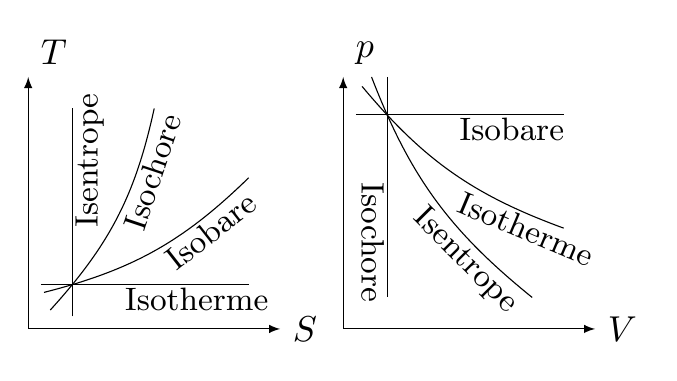
\begin{tikzpicture}
	[
	scale=0.8, every node/.style={scale=1.3},
	> = latex,
	dot/.style = {draw,fill,circle,inner sep=1pt},
	arrow inside/.style = {postaction=decorate,decoration={markings,mark=at position .55 with \arrow{>}}}
	]
  	\draw[<->] (0,4) node[above right] {$T$} |- (4,0) node[right] {$S$};
  	\draw[<->] (5,4) node[above right] {$p$} |- (9,0) node[right] {$V$};

	\draw (0.7,0.2) to node[near end, below=-1.2mm, sloped] {\small Isentrope} (0.7,3.5);
	\draw (0.2,0.7) to node[near end, below=-1.2mm, sloped] {\small Isotherme} (3.5,0.7);
	\draw (0.35,0.3) to[bend right=15] node[near end, below=-1.2mm, sloped] {\small Isochore} (2,3.5);
	\draw (0.25,0.58) to[bend right=15] node[near end, below=-1.2mm, sloped] {\small Isobare} (3.5,2.4);

	\draw (5.7,4) to node[near end, below=-1.2mm, sloped] {\small Isochore} (5.7,0.5);
	\draw (5.2,3.4) to node[near end, below=-1.2mm, sloped] {\small Isobare} (8.5,3.4);
	\draw (5.45,4) to[bend right=15] node[near end, below=-1.2mm, sloped] {\small Isentrope } (8,0.5);
	\draw (5.3,3.85) to[bend right=15] node[very near end, below=-1.2mm, sloped] {\small Isotherme} (8.5,1.6);
\end{tikzpicture}
%   _______ __    __        
%  / ____(_) /_  / /_  _____
% / / __/ / __ \/ __ \/ ___/
%/ /_/ / / /_/ / /_/ (__  )
%\____/_/_.___/_.___/____/
\section{Gibbs}

\begin{align*}
	dU &=  TdS - pdV + \sum_{k=1}^{K} \mu_k dn_k \\
	dG &= -SdT + Vdp + \sum_{k=1}^{K} \mu_k dn_k \\ dH &=  TdS + Vdp + \sum_{k=1}^{K} \mu_k dn_k \\
	dF &= -SdT - pdV + \sum_{k=1}^{K} \mu_k dn_k \\
	dU &= 	\left(\frac{\partial U}{\partial S}\right)_{V} dS 
	+ 	\left(\frac{\partial U}{\partial V}\right)_{S} dV 
	+ 	\sum_{k=1}^{K} \left(\frac{\partial U}{\partial n_k}\right)_{S} dn_k  \\
\end{align*}


%    ____             _      __                               
%   / __ )___  ____  (_)__  / /_  __  ______  ____ ____  ____ 
%  / __  / _ \/_  / / / _ \/ __ \/ / / / __ \/ __ `/ _ \/ __ \
% / /_/ /  __/ / /_/ /  __/ / / / /_/ / / / / /_/ /  __/ / / /
%/_____/\___/ /___/_/\___/_/ /_/\__,_/_/ /_/\__, /\___/_/ /_/ 
%                                          /____/             
\section{Thermodynamische Beziehungen}

\begin{multicols}{2}

\begin{align*}
	T   	&= \quad \left(\frac{\partial U}{\partial S}\right)_{V} = T(S,V)  	\\
	T   	&= \quad \left(\frac{\partial H}{\partial S}\right)_{p} = T(S,p)  	\\
	p   	&= -\left(\frac{\partial U}{\partial V}\right)_{S} = p(V,S)	      	\\
	-p  	&= \quad \left(\frac{\partial F}{\partial V}\right)_{T} = p(T,V)	\\
		%\left(\frac{\partial u}{\partial v}\right)_{T} &= T\left(\frac{\partial p}{\partial T}\right)_{v} -p
\end{align*}

\begin{align*}
	-S 	&= \left(\frac{\partial F}{\partial T}\right)_{V} = S(T,V)		\\
	-S 	&= \left(\frac{\partial G}{\partial T}\right)_{p} = S(T,p)		\\
	 V 	&= \left(\frac{\partial G}{\partial p}\right)_{T} = V(p,T)		\\
	\mu 	&= \left(\frac{\partial U}{\partial n}\right)_{S,V} = \mu(S,V,n)	\\
\end{align*}
\end{multicols}

%   ______                             __         _         
%  / ____/_  ______ _____ ____  ____  / /_  ___  (_)___ ___ 
% / / __/ / / / __ `/ __ `/ _ \/ __ \/ __ \/ _ \/ / __ `__ \
%/ /_/ / /_/ / /_/ / /_/ /  __/ / / / / / /  __/ / / / / / /
%\____/\__,_/\__, /\__, /\___/_/ /_/_/ /_/\___/_/_/ /_/ /_/ 
%           /____//____/                                    

\section{Guggenheim}
\Large
\begin{tabular}{llllll}
	-S & U & V &	&U &= U(S,V) \\ 
	 H &   & F &   	&H &= H(S,p) \\
	-p & G & T &   	&F &= F(T,V) \\
	   &   &   &  	&G &= G(T,p) \\
\end{tabular}
\normalsize
\ultraskip
\pagebreak


%    __  ___                         ____
%   /  |/  /___ __  ___      _____  / / /
%  / /|_/ / __ `/ |/_/ | /| / / _ \/ / / 
% / /  / / /_/ />  < | |/ |/ /  __/ / /  
%/_/  /_/\__,_/_/|_| |__/|__/\___/_/_/   

\section{Maxwell}

\begin{align*}
	\left(\frac{\partial T}{\partial p}\right)_{S,n_j}
	&= \quad
	\left(\frac{\partial V}{\partial S}\right)_{p,n_j}
	\\\\
	\left(\frac{\partial S}{\partial V}\right)_{T,n_j}
	&= \quad
	\left(\frac{\partial p}{\partial T}\right)_{V,n_j}
	\\\\
	\left(\frac{\partial S}{\partial p}\right)_{T,n_j}
	&= -
	\left(\frac{\partial V}{\partial T}\right)_{p,n_j}
	\\\\
	\left(\frac{\partial \mu _i}{\partial T}\right)_{p,n_j}
	&= -
	\left(\frac{\partial S}{\partial n_i}\right)_{T,p,n_j \neq n_i}
	\\\\
	\left(\frac{\partial \mu_i}{\partial p}\right)_{T,n_j}
	&=
	\quad \left(\frac{\partial V}{\partial n_i}\right)_{T,p,n_j \neq n_i}
\end{align*}

%    ____    __           __             ______          
%   /  _/___/ /__  ____ _/ /__  _____   / ____/___ ______
%   / // __  / _ \/ __ `/ / _ \/ ___/  / / __/ __ `/ ___/
% _/ // /_/ /  __/ /_/ / /  __(__  )  / /_/ / /_/ (__  ) 
%/___/\__,_/\___/\__,_/_/\___/____/   \____/\__,_/____/  
                                                        
\section{Ideales Gas}
\setlength{\belowdisplayskip}{-10pt} \setlength{\belowdisplayshortskip}{-10pt}

\begin{align*}
	&pV = mRT \\ 
	&pv = RT \\
	&pV = nR_mT \\
	&\beta = \frac{1}{T} \\
	&\gamma = \frac{1}{T} \\
	&\chi = \frac{1}{p} \\
	&\beta = p \gamma \chi\\
	&R_m = 8,3143\left[\frac{kJ}{kmolK}\right] \\
	&R = c_p - c_v\\
	&R = \frac{R_m}{M}
	\\
	&U - U_0 = mc_v(T-T_0)
	\\
	&H - H_0 = mc_p(T-T_0) \quad \leftarrow \text{Für $c_p$ und $c_v$ const.}
\end{align*}
\begin{alignat*}{3}
	&s - s_0 
	&&= R \ln \left(\frac{ v}{ v_0}\right)_{} 
	&&+ c_v \ln \left(\frac{ T}{ T_0}\right)_{}
	\\
	& 
	&&= c_v \ln \left( \frac{p}{p_0} \right) 
	&&+ c_p \ln \left( \frac{v}{v_0} \right)
	\\
	& 
	&&= c_p \ln \left( \frac{T}{T_0} \right) 
	&&-R \ln \left( \frac{p}{p_0} \right)
	\\
	&\beta 
	= \frac{1}{T} 
	&&=\frac{1}{V}\left(\frac{\partial V}{\partial T}\right)_{p} 
	&&=  \frac{1}{v}\left(\frac{\partial v}{\partial T}\right)_{p} 
	=  - \frac{1}{\rho}\left(\frac{\partial \rho}{\partial T}\right)_{p} 
	\\
	&\gamma 
	= \frac{1}{T}  
	&&= \frac{1}{p} \: \left(\frac{\partial p}{\partial T}\right)_{V}
	\\
	&\chi 
	= \frac{1}{p} 
	&&= - \frac{1}{V}\left(\frac{\partial V}{\partial p}\right)_{T}  
	&&= - \frac{1}{v}\left(\frac{\partial v}{\partial p}\right)_{T}
	\\
		& u_2 - u_1 &&= \int_{T_1}^{T_2} c_v(T)\; dT
	\\
	& U_2 - U_1 &&= Q_{12} + W_{V,12} \\
\end{alignat*}
% _    __                      __              _       __            __    
%| |  / /___ _____        ____/ /__  _____    | |     / /___ _____ _/ /____
%| | / / __ `/ __ \______/ __  / _ \/ ___/____| | /| / / __ `/ __ `/ / ___/
%| |/ / /_/ / / / /_____/ /_/ /  __/ /  /_____/ |/ |/ / /_/ / /_/ / (__  ) 
%|___/\__,_/_/ /_/      \__,_/\___/_/         |__/|__/\__,_/\__,_/_/____/  
                                                                          
\section{Van-der-Waals}
\begin{align*}
	&\left(p + \frac{a}{v^2}\right)(v-b) = RT 
	\\
	&\left(\overline{p} + \frac{3}{\overline{v}^2}\right)(3\overline{v}-1) = 8\overline{T} 
	\\
	&\overline{p} = \frac{p}{p_K}, \quad \overline{v} = \frac{v}{v_K}, \quad \overline{T} = \frac{T}{T_K} 
	\\
	&p_K = \frac{a}{27b^2}, \quad T_K = \frac{8}{27}\frac{a}{b}\frac{1}{R}, \quad %\xrightswishingghost{} 
	\\
	&a=3p_Kv^2_K, \quad b =\frac{v_K}{3}, \quad \frac{p_Kv_K}{RT_K} = \frac{3}{8} 
	\\
	&\beta = \frac{(v-b)Rv^2}{RTv^3 - 2a(v-b)^2} 
	\\ 
	&\gamma = \frac{Rv^2}{RTv^2 - a(v-b)} 
	\\
	&\chi = \frac{(v-b)^2v^2}{RTv^3 - 2a(v-b)^2} 
	\\
	& du = \frac{a}{v^2}dv + c_v(T)dT 
	\\
	&u-u_0 = \left( \frac{a}{v_0} - \frac{a}{v} \right) + \int_{T_0}^{T} c_v(\tilde{T})\; d\tilde{T} 
	\\
	& u - u_0 = \left(\frac{a}{v_0} - \frac{a}{v} \right) + c_v(T-T_0) \leftarrow \text{für $c_v$ = const.} 
	\\
	&c_p - c_v = \frac{Tv\beta^2}{\chi} 
	\\
	& s- s_0 = c_v \ln \left( \frac{T}{T_0} \right) + R \ln \left(\frac{v-b}{v_0 - b} \right)
	\\
	& h_2 - h_1 = \frac{1}{2}(p_2 - p_1) \left( \frac{1}{\rho_1} + \frac{1}{\rho_2}\right)
	\\
\end{align*}

%    ____                            __                 
%   / __ \_________  _____________  / /_  ______  ____ _
%  / / / / ___/ __ \/ ___/ ___/ _ \/ / / / / __ \/ __ `/
% / /_/ / /  / /_/ (__  |__  )  __/ / /_/ / / / / /_/ / 
%/_____/_/   \____/____/____/\___/_/\__,_/_/ /_/\__, /  
%                                              /____/   
\section{Drosselung}

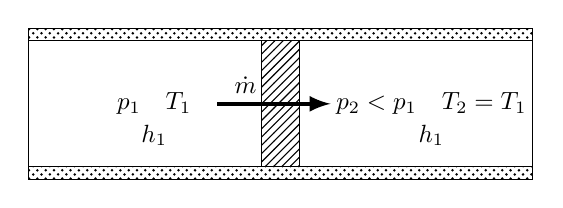
\begin{tikzpicture}
	[
	scale=0.8, every node/.style={scale=0.9},
	> = latex,
	dot/.style = {draw,fill,circle,inner sep=1pt},
	arrow inside/.style = {postaction=decorate,decoration={markings,mark=at position .55 with \arrow{>}}}
	]
	\draw (0,0) to (0,2) to (8,2) to (8,0) to (0,0);
	\draw[pattern=crosshatch dots] (0,0) to (0,-0.2) to (8,-0.2) to (8,0) to (0,0);
	\draw[pattern=crosshatch dots] (0,2) to (0,2.2) to (8,2.2) to (8,2) to (0,2);
	\draw[pattern=north east lines] (3.7,2) to (4.3,2) to (4.3,0) to (3.7,0) to (3.7,2);

	\draw (2,1) node {$p_1 \quad T_1$};
	\draw (2,0.5) node {$h_1$};
	\draw (6.4,1) node {$p_2 < p_1 \quad T_2 = T_1$};
	\draw (6.4,0.5) node {$h_1$};
	\draw[->,ultra thick] (3,1) to node[near start, above] {$\dot{m}$} (4.8,1);
\end{tikzpicture}
\begin{align*}
	& h + \frac{c^2}{2} + gz = \text{const.} \\
	& dh = 0, \quad T_1 = T_2 \\
	& \delta_h = \left(\frac{\partial T}{\partial p}\right)_{h}  = - \frac{v}{c_p}(1-\beta T) \\
	& \delta_T = \left(\frac{\partial h}{\partial p}\right)_{T}  \\
	& s_2 - s_1 = R \ln \left(\frac{v_2}{v_1}\right) = R \ln \left( \frac{p_1}{p_2}\right) \\
	&\mu_{J-T} = \left(\frac{\partial H}{\partial p}\right)_{H} \approx \frac{\frac{2a}{RT}-b}{c_{p,m}}  \\
	&T_i = \frac{2a}{Rb}  \\
\end{align*}

\pagebreak

%   ______                       __ 
%  / ____/___ __________  ____  / /_
% / /   / __ `/ ___/ __ \/ __ \/ __/
%/ /___/ /_/ / /  / / / / /_/ / /_  
%\____/\__,_/_/  /_/ /_/\____/\__/  

\section{Carnot}

\begin{align*}
	&\eta_{th} = 1 - \frac{-Q_{34}}{Q_{12}} 
	= 1 - \frac{T_3(S_3-S_4)}{T_1(S_2 - S_1)} 
	= 1 - \frac{T_1}{T_3} \\
	&\frac{Q_{12}}{T_1} + \frac{Q_{34}}{T_3} 
	= 0 \\
	&\Delta S_{ges} 
	= -Q_{34} \left( \frac{1}{T_{KK}} 
	- \frac{T_1}{T_3}\frac{1}{T_{HK}} \right)
\end{align*}

\bigskip 

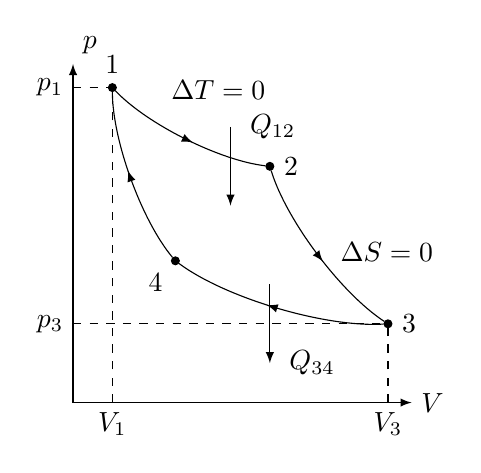
\begin{tikzpicture}[
  > = latex,
  dot/.style = {draw,fill,circle,inner sep=1pt},
  arrow inside/.style = {postaction=decorate,decoration={markings,mark=at position .55 with \arrow{>}}}
  ]
  \draw[<->] (0,4.3) node[above right] {$p$} |- (4.3,0) node[right] {$V$};
  \node[dot,label={above:$1$}] (@1) at (0.5,4) {};
  \node[dot,label={right:$2$}] (@2) at (2.5,3) {};
  \node[dot,label={right:$3$}] (@3) at (4,1) {};
  \node[dot,label={below left:$4$}] (@4) at (1.3,1.8) {};

  \node[label={above right:$\Delta T = 0$}] at (1,3.6) {};
  \node[label={above right:$\Delta S = 0$}] at (3.15,1.54) {};

  \draw[arrow inside] (@1) to[looseness=.7,bend right=20] (@2);
  \draw[arrow inside] (@2) to[looseness=.7,bend right=20] (@3);
  \draw[arrow inside] (@3) to[looseness=.7,bend left=20] (@4);
  \draw[arrow inside] (@4) to[looseness=.7,bend left=20] (@1);
  \draw[dashed,thin] (0,4) node[left] {$p_1$} -- (0.5,4);
  \draw[dashed,thin] (0,1) node[left] {$p_3$} -- (4,1);
  \draw[dashed,thin] (0.5,0) node[below] {$V_1$} -- (0.5,4);
  \draw[dashed,thin] (4,0) node[below] {$V_3$} -- (4,1);

  \draw[->] (2,3.5) to (2,2.5);
  \node[label={right:$Q_{12}$}] at (2,3.5) {};
  \draw[->] (2.5,1.5) to (2.5,0.5);
  \node[label={right:$Q_{34}$}] at (2.5,0.5) {};
\end{tikzpicture}

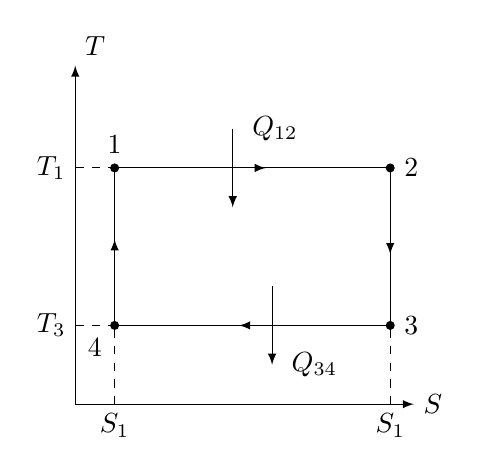
\begin{tikzpicture}[
  > = latex,
  dot/.style = {draw,fill,circle,inner sep=1pt},
  arrow inside/.style = {postaction=decorate,decoration={markings,mark=at position .55 with \arrow{>}}}
  ]
  \draw[<->] (0,4.3) node[above right] {$T$} |- (4.3,0) node[right] {$S$};
  \node[dot,label={above:$1$}] (@1) at (0.5,3) {};
  \node[dot,label={right:$2$}] (@2) at (4,3) {};
  \node[dot,label={right:$3$}] (@3) at (4,1) {};
  \node[dot,label={below left:$4$}] (@4) at (0.5,1) {};

  \draw[arrow inside] (@1) to (@2);
  \draw[arrow inside] (@2) to (@3);
  \draw[arrow inside] (@3) to (@4);
  \draw[arrow inside] (@4) to (@1);
  \draw[dashed,thin] (0,3) node[left] {$T_1$} -- (0.5,3);
  \draw[dashed,thin] (0,1) node[left] {$T_3$} -- (0.50,1);
  \draw[dashed,thin] (0.5,0) node[below] {$S_1$} -- (0.5,1);
  \draw[dashed,thin] (4,0) node[below] {$S_1$} -- (4,1);

  \draw[->] (2,3.5) to (2,2.5);
  \node[label={right:$Q_{12}$}] at (2,3.5) {};
  \draw[->] (2.5,1.5) to (2.5,0.5);
  \node[label={right:$Q_{34}$}] at (2.5,0.5) {};
\end{tikzpicture}

%   ______               _           __       
%  / ____/__  ____ ___  (_)_________/ /_  ___ 
% / / __/ _ \/ __ `__ \/ / ___/ ___/ __ \/ _ \
%/ /_/ /  __/ / / / / / (__  ) /__/ / / /  __/
%\____/\___/_/ /_/ /_/_/____/\___/_/ /_/\___/ 
%                                             
%    ____    __           __             ______              
%   /  _/___/ /__  ____ _/ /__  _____   / ____/___ _________ 
%   / // __  / _ \/ __ `/ / _ \/ ___/  / / __/ __ `/ ___/ _ \
% _/ // /_/ /  __/ /_/ / /  __/ /     / /_/ / /_/ (__  )  __/
%/___/\__,_/\___/\__,_/_/\___/_/      \____/\__,_/____/\___/ 
                                                            
\section{Gemische Idealer Gase}

\begin{align*}
	&\xi_i
	= \frac{m_i}{m}, \quad \psi_i
	= \frac{n_i}{n}, \quad p_i
	= \psi_ip \\
	&\xi_i
	= \frac{M_i n_i}{\sum_{k
	= 1}^{K} M_kn_k}
	= \frac{M_i}{M_G}\psi  
	\\
	& p_iV
	= m_iR_iT, \quad p_iV
	= n_iR_mT, \quad pV
	= mR_GT \\
	& \sum_{k
	= 1}^{K} p_k
	= p 
	\\
	&R_G
	= \frac{1}{m} \sum_{k=1}^{K} m_kR_k
	= \sum_{k=1}^{K} \xi_k R_k 
	\\
	&U_G
	= \sum_{k=1}^{K} U_k
	= \sum_{k=1}^{K} m_k u_k
	= \sum_{k=1}^{K} c_{vk}m_kT \leftarrow \text{$c_v$
	= const}
	\\
	&H_G
	= \sum_{k=1}^{K} H_k
	= \sum_{k=1}^{K} m_k h_k
	= \sum_{k=1}^{K} c_{pk}m_kT \leftarrow \text{$c_p$
	= const.}
	\\
	&c_{vG}
	= \sum_{k=1}^{K} c_{vk} \xi_k, \quad c_{pG}
	= \sum_{k=1}^{K} c_{pk}\xi_k 
	\\
	&S_2-S_1
	= R_m \left( n \ln n - \sum_{k=1}^{K} n_k \ln n_k \right)
\end{align*}


%    _   __                    __                      ____
%   / | / /___ _______________/ /___ _____ ___  ____  / __/
%  /  |/ / __ `/ ___/ ___/ __  / __ `/ __ `__ \/ __ \/ /_  
% / /|  / /_/ (__  |__  ) /_/ / /_/ / / / / / / /_/ / __/  
%/_/ |_/\__,_/____/____/\__,_/\__,_/_/ /_/ /_/ .___/_/     
%                                           /_/            

\section{Nassdampf}
\tiny
\begin{flushleft}
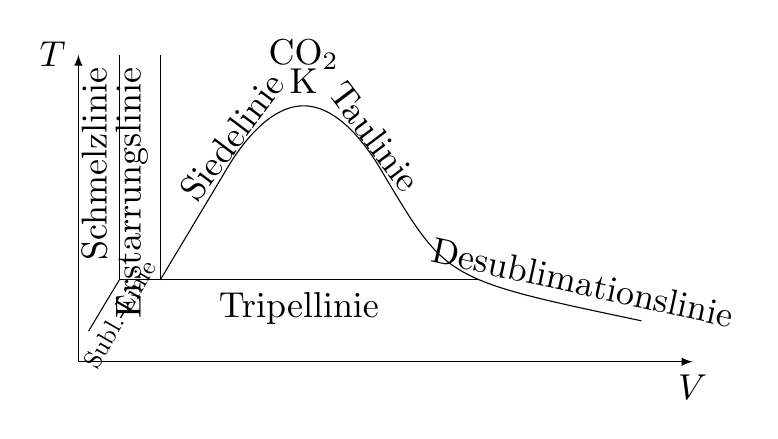
\begin{tikzpicture}
	[
	scale=1.3, every node/.style={scale=1.3},
	> = latex,
	dot/.style = {draw,fill,circle,inner sep=1pt},
	arrow inside/.style = {postaction=decorate,decoration={markings,mark=at position .55 with \arrow{>}}}
	]
	\draw[<->]  (0,3) node[left] {$T$} |- (6,0) node[below] {$V$} ;
	\draw (0.1,0.3) -- node[midway, below, rotate=60, scale=0.7] {Subl.-Linie} (0.4,0.8);
	\draw (0.4, 0.8) -- (0.4, 3) node[above left, rotate=90] {Schmelzlinie};
	\draw (0.8, 0.8) -- (0.8, 3) node[above left, rotate=90] {Erstarrungslinie};
	\draw (0.4,0.8) -- node[midway, below] {Tripellinie} (3.91,0.8);
	\draw (0.8,0.8) -- (1.4,1.8);
	\draw (1.4,1.8) parabola bend (2.2,2.5) (3,1.8);
	\draw (3,1.8)  .. controls (3.6,0.8) .. node[very near end, sloped, above] {Desublimationslinie} (5.5,0.4);
	\draw (1.5,2.2) node[rotate=53] {Siedelinie};
	\draw (2.9,2.2) node[rotate=-53] {Taulinie};
	\draw (2.2,3) node {$\text{CO}_\text{2}$};
	\draw (2.2,2.5) node[above] {K};
\end{tikzpicture}

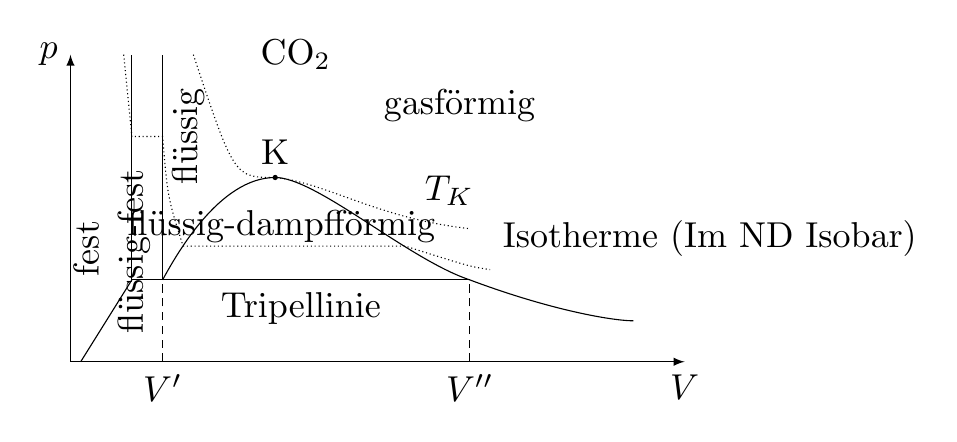
\begin{tikzpicture}
	[
	scale=1.3, every node/.style={scale=1.3},
	> = latex,
	dot/.style = {draw,fill,circle,inner sep=1pt},
	arrow inside/.style = {postaction=decorate,decoration={markings,mark=at position .55 with \arrow{>}}}
	]
	\draw[<->]  (0,3) node[left] {$p$} |- (6,0) node[below] {$V$} ;
	\draw (0.1,0) -- (0.6,0.8);
	\draw (0.6, 0.8) -- (0.6, 3) ;
	\draw (0.9, 0.8) -- (0.9, 3);
	\draw (0.6,0.8) -- node[midway, below] {Tripellinie} (3.9,0.8);

	\draw (0.9,0.8) parabola[bend at end]  (2, 1.8);

	\draw (2,1.8) .. controls (2.4,1.8) and (3.3, 1) .. (3.9,0.8) .. controls (4.7,0.5) and (5.3,0.4) .. (5.5,0.4);
	%\draw (2,1.8) .. controls (2.4,1.8) and (3.3, 1) .. (3.9,0.8) .. controls (4.7,0.5) and (5.3,0.4) .. node[above, sloped]  {$\xrightswishingghost{}$} (5.5,0.4);
	\draw (2.2,3) node {$\text{CO}_\text{2}$};

	\draw[fill] (2,1.8) circle (0.02) node[above] {K};

	\draw[densely dashed] (0.9,0) node[below] {$V'$} -- (0.9,0.8);
	\draw[densely dashed] (3.9,0) node[below] {$V''$} -- (3.9,0.8);
	\draw (3.7,1.4) node[above]  {$T_K$};
	\draw (0.4,1.5) node[above left, rotate=90] {fest};
	\draw (1.15,2.2) node[rotate=90] {flüssig};
 	\draw (0.9,2) node[above left, rotate=90] {flüssig-fest};
	\draw (2.06,1.32) node {flüssig-dampfförmig};
	\draw (3.8,2.5) node {gasförmig};

	\draw[densely dotted] (1.2,3) ..controls (1.6,1.8) .. (2,1.8) .. controls(2.5,1.75) and (3,1.4) .. (3.9, 1.3);
	\draw[densely dotted] (0.52,3) to (0.6,2.2) to (0.6,2.2) to (0.9,2.2) .. controls (0.95,1.6) .. (1.1,1.13) -- (3.27,1.13) .. controls (3.9,0.93) .. (4.1,0.9) node[above right] {Isotherme (Im ND Isobar)};
\end{tikzpicture}

\begin{center}
\large H$_2$O \\
\end{center}

\begin{multicols}{2}
\normalsize


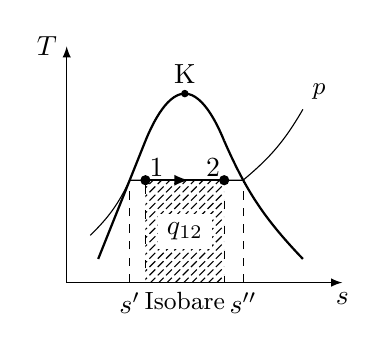
\begin{tikzpicture}
	[> = latex,
	scale=1.0, every node/.style={scale=1},
	dot/.style = {draw,fill,circle,inner sep=1pt},
	arrow inside/.style = {postaction=decorate,decoration={markings,mark=at position .55 with \arrow{>}}}
	]
	\coordinate (a) at (0.4,0.3);
	\coordinate (b) at (1.0,1.8);
	\coordinate (c) at (1.5,2.4);
	\coordinate (d) at (2.0,1.8);
	\coordinate (e) at (3.0,0.3);
	\coordinate (f) at (0.3,0.6);
	\coordinate (g) at (0.8,1.3);
	\coordinate (h) at (2.24,1.3);
	\coordinate (i) at (3,2.2);
	\coordinate (j) at (0.3,0.7);
	\coordinate (k) at (0.9,1.57);
	\coordinate (l) at (2.10,1.57);
	\coordinate (m) at (2.5,2.15);

	\draw[<->]  (0,3) node[left] {$T$} |- (3.5,0) node[below] {$s$};
	\draw[thick, name path=patha] (a) -- (b);
	\draw[thick] (b) parabola bend (c) (2,1.8);
	\draw[thick] (2,1.8) to[bend right=10] (3,0.3);

	\draw[fill] (c) circle (0.04) node[above] {K};

	\draw[] (f) to[bend right=10] (g) to (h) to[bend right=10] (i) node[above right] {\small $p$};

	\draw[thick, arrow inside] (1,1.3) node[dot] {} to (2,1.3) node[dot] {};
	\draw[pattern=north east lines, loosely dashed] (1,1.3) to (2,1.3) to (2,0) to (1,0) to (1,1.3);
	\draw (1.5,0.65) node[fill=white] {$q_{12}$};
	\draw (1,1.3) node[above right=-1mm] {1};
	\draw (2,1.3) node[above left=-1mm] {2};

	\draw (1.5,0) node[below] {\small Isobare};
	\draw[dashed] (0.8,0) node[below] {$s'$} to (g);
	\draw[dashed] (2.24,0) node[below] {$s''$} to (h);
\end{tikzpicture}

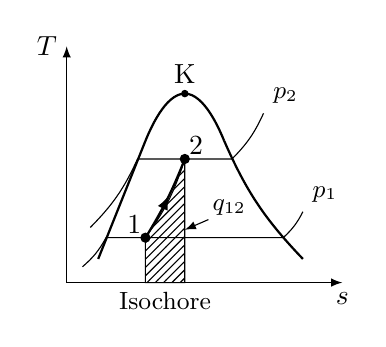
\begin{tikzpicture}
	[> = latex,
	scale=1.0, every node/.style={scale=1},
	dot/.style = {draw,fill,circle,inner sep=1pt},
	arrow inside/.style = {postaction=decorate,decoration={markings,mark=at position .55 with \arrow{>}}}
	]
	\coordinate (a) at (0.4,0.3);
	\coordinate (b) at (1.0,1.8);
	\coordinate (c) at (1.5,2.4);
	\coordinate (d) at (2.0,1.8);
	\coordinate (e) at (3.0,0.3);
	\coordinate (f) at (0.2,0.2);
	\coordinate (g) at (0.5,0.57);
	\coordinate (h) at (2.75,0.57);
	\coordinate (i) at (3,0.9);
	\coordinate (j) at (0.3,0.7);
	\coordinate (k) at (0.9,1.57);
	\coordinate (l) at (2.10,1.57);
	\coordinate (m) at (2.5,2.15);

	\draw[<->]  (0,3) node[left] {$T$} |- (3.5,0) node[below] {$s$};
	\draw[thick, name path=patha] (a) -- (b);
	\draw[thick] (b) parabola bend (c) (d);
	\draw[thick] (d) to[bend right=10] (e);

	\draw[fill] (c) circle (0.04) node[above] {K};

	\draw[] (f) to[bend right=10] (g) to (h) to[bend right=10] (i) node[above right] {\small $p_1$};
	\draw[] (j) to[bend right=10] (k) to (l) to[bend right=10] (m) node[above right] {\small $p_2$};

	\draw[arrow inside, thick] (1,0.57) node[draw, dot] {} to[bend right=5] (1.5,1.57) node[draw, dot] {};
	\draw[pattern=north east lines] (1,0.57) node[above left=-1mm] {1} to[bend right=9] (1.5,1.57) node[above right=-1mm] {2} to (1.5,0) to (1,0) to (1,0.57);
	\draw[<-] (1.5,0.67) to  (1.8,0.8) node[above right=-1mm] {\small $q_{12}$};
	\draw (1.25,0) node[below] {\small Isochore};
\end{tikzpicture}
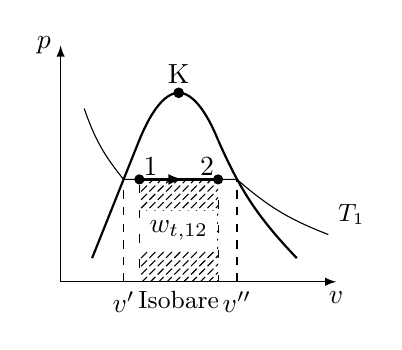
\begin{tikzpicture}
	 [> = latex,
	scale=1.0, every node/.style={scale=1},
	dot/.style = {draw,fill,circle,inner sep=1pt},
	arrow inside/.style = {postaction=decorate,decoration={markings,mark=at position .55 with \arrow{>}}}
	]
	\coordinate (a) at (0.4,0.3);
	\coordinate (b) at (1.0,1.8);
	\coordinate (c) at (1.5,2.4);
	\coordinate (d) at (2.0,1.8);
	\coordinate (e) at (3.0,0.3);
	\coordinate (f) at (0.2,0.2);
	\coordinate (g) at (0.8,1.3);
	\coordinate (h) at (2.24,1.3);
	\coordinate (i) at (3,2.2);
	\coordinate (j) at (0.3,0.7);
	\coordinate (k) at (0.9,1.57);
	\coordinate (l) at (2.10,1.57);
	\coordinate (m) at (2.5,2.15);

	\draw[<->]  (0,3) node[left] {$p$} |- (3.5,0) node[below] {$v$};
	\draw[thick, name path=patha] (a) -- (b);
	\draw[thick] (b) parabola bend (c) (2,1.8);
	\draw[thick] (2,1.8) to[bend right=10] (3,0.3);

	\draw[fill] (c) circle (0.06) node[above] {K};

	\draw[] (0.3,2.2) to[bend right=10] (g) to (h) to[bend right=10] (3.4,0.6) node[above right] {\small $T_1$};
	\draw[thick, arrow inside] (1,1.3) node[dot] {} to (2,1.3) node[dot] {};
	\draw[pattern=north east lines, loosely dashed] (1,1.3) to (2,1.3) to (2,0) to (1,0) to (1,1.3);
	\draw (1.5,0.65) node[fill=white] {$w_{t,12}$};
	\draw (1,1.3) node[above right=-1mm] {1};
	\draw (2,1.3) node[above left=-1mm] {2};
	\draw (1.5,0) node[below] {\small Isobare};

	\draw[dashed] (0.8,0) node[below] {$v'$} to (g);
	\draw[dashed] (2.24,0) node[below] {$v''$} to (h);
\end{tikzpicture}

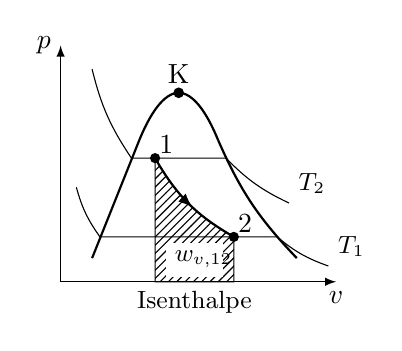
\begin{tikzpicture}
	 [> = latex,
	scale=1.0, every node/.style={scale=1},
	dot/.style = {draw,fill,circle,inner sep=1pt},
	arrow inside/.style = {postaction=decorate,decoration={markings,mark=at position .55 with \arrow{>}}}
	]
	\coordinate (a) at (0.4,0.3);
	\coordinate (b) at (1.0,1.8);
	\coordinate (c) at (1.5,2.4);
	\coordinate (d) at (2.0,1.8);
	\coordinate (e) at (3.0,0.3);
	\coordinate (f) at (0.2,0.2);
	\coordinate (g) at (0.5,0.57);
	\coordinate (h) at (2.75,0.57);
	\coordinate (i) at (3,0.9);
	\coordinate (j) at (0.3,0.7);
	\coordinate (k) at (0.9,1.57);
	\coordinate (l) at (2.10,1.57);
	\coordinate (m) at (2.5,2.15);

	\draw[<->]  (0,3) node[left] {$p$} |- (3.5,0) node[below] {$v$};
	\draw[thick, name path=patha] (a) -- (b);
	\draw[thick] (b) parabola bend (c) (2,1.8);
	\draw[thick] (2,1.8) to[bend right=10] (3,0.3);

	\draw[fill] (c) circle (0.06) node[above] {K};

	\draw[] (0.2,1.2) to[bend right=10] (g) to (h) to[bend right=10] (3.4,0.2) node[above right] {\small $T_1$};
	\draw[] (0.4,2.7) to[bend right=10] (k) to (l) to[bend right=10] (2.9,1) node[above right] {\small $T_2$};
	
	\draw[thick, arrow inside] (1.2,1.57) node[draw, dot] {} to[bend right=15] (2.2,0.57) node[draw, dot] {};
	\draw[pattern=north east lines] (1.2,1.57) node[above right=-1mm] {1} to[bend right=15] (2.2,0.57) node[above right=-1mm] {2} to (2.2,0) to (1.2,0) to (1.2,1.57);
	\draw (1.7,0.28) node[fill=white, text width=5mm, text height=1.2mm, align=left] {\small $w_{v,12}$};
	\draw (1.7,0) node[below] {\small Isenthalpe};
\end{tikzpicture}
\end{multicols}

\end{flushleft}
\large
\begin{equation*}
	\frac{dp}{dT} = \frac{s'' - s'}{v'' - v'} = \frac{1}{T}\frac{h'' - h'}{v'' - v'} 
\end{equation*}
\normalsize
\begin{multicols}{2}
\begin{align*}
	& r = h'' - h' = T(s''-s') \\
	& v = (1-x)v' + xv{''} \\
	& v = v' + (v''-v')x \\ 
	& u = (1-x) u' + xu'' \\
	& u = u' + (u''-u')x \\
	& h = (1-x) h' + xh'' \\
	& h = h' + (h''-h')x \\
	& s = (1-x) s' + xs'' \\
	& s = s' + (s''-s')x \\
\end{align*}

\begin{align*}
	& \frac{dp}{dT} = \frac{1}{T}\frac{r}{v'' -v'}  \\
	& F  = K + 2 - P \\
	& T' = T'' \\
	& p' = p'' \\
	& g' = g'' \\
	&dg' = v'dp' - s'dT' \\
	&dg'' = v'' dp'' - s'' dT'' \\
	&dg' = dg'' \\
\end{align*}
\end{multicols}


%    ____             __             _____ __        ________   _         
%   / __ \___  ____ _/ /__  _____   / ___// /_____  / __/ __/  (_)___ ___ 
%  / /_/ / _ \/ __ `/ / _ \/ ___/   \__ \/ __/ __ \/ /_/ /_   / / __ `__ \
% / _, _/  __/ /_/ / /  __/ /      ___/ / /_/ /_/ / __/ __/  / / / / / / /
%/_/ |_|\___/\__,_/_/\___/_/      /____/\__/\____/_/ /_/    /_/_/ /_/ /_/ 
%                                                                         
%    _   __                    __                      ____           __    _      __
%   / | / /___ _______________/ /___ _____ ___  ____  / __/___  ___  / /_  (_)__  / /
%  /  |/ / __ `/ ___/ ___/ __  / __ `/ __ `__ \/ __ \/ /_/ __ `/ _ \/ __ \/ / _ \/ _/
% / /|  / /_/ (__  |__  ) /_/ / /_/ / / / / / / /_/ / __/ /_/ /  __/ /_/ / /  __/ /__
%/_/ |_/\__,_/____/____/\__,_/\__,_/_/ /_/ /_/ .___/_/  \__, /\___/_.___/_/\ __/\___/
%                                           /_/        /____/                 

\section{Realer Stoff im Nassdampfgebiet}
\begin{align*}
	\text{Isobare } &\text{Zustandsänderung} \\
	q_{12} &= T(s_2 - s_1) \\
	&= T\Big(s'' - s'\Big)(x_2-x_1) \\
	w_{V,12} &= - \int_{1}^{2} p\; dv \\
	&= -p(v_2-v_1) = -p\Big(v'' -v'\Big)(x_2-x_1) \\
	\text{Isochore } &\text{Zustandsänderung} \\
	q_{12} &= u_2 - u_1 = u_2' + x_2\Big(u_2'' - u_2' \Big) - u_1' - x_1\Big(u_1'' - u_1'\Big) \\
	\text{Adiabate } &\text{Zustandsänderung} \\
	w_{V,12} &= u_2 - u_1 = u_2' + x_2 \Big( u_2'' - u_2' \Big) - u_1' - x_1\Big(u_1'' - u_1'\Big) \\
	\text{Entropie} & \text{Änderung während des Mischvorgangs} \\
	&S_2-S_1 = R_m \left ( n \ln n - \sum_{i}^{} n_i \ln n_i \right ) \\
\end{align*}

%    ______                     _    
%   / ____/  _____  _________ _(_)__ 
%  / __/ | |/_/ _ \/ ___/ __ `/ / _ \
% / /____>  </  __/ /  / /_/ / /  __/
%/_____/_/|_|\___/_/   \__, /_/\___/ 
%	              /____/         

\section{Maximale Arbeit und Exergie}
Maximal nutzbare Arbeit $\rightarrow$ isentrop, reibungsfrei \\
$1 \rightarrow 1'$ : isentrop auf $T_u$ \\
$1' \rightarrow u$ : isotherm auf $u$ 

\begin{multicols}{2}


	\begin{flushleft}

\begin{tikzpicture}[
	scale=0.8, every node/.style={scale=1},
  > = latex,
  dot/.style = {draw,fill,circle,inner sep=1pt},
  arrow inside/.style = {postaction=decorate,decoration={markings,mark=at position .55 with \arrow{>}}}
  ]
  	\draw[<->] (0,4.3) node[above right] {$T$} |- (4.3,0) node[right] {$S$};

	\coordinate (a) at (0.8,0.6);
	\coordinate (b) at (0.8,2);

	\coordinate (c) at (3.3,3.5);
	\coordinate (d) at (3.3,2);

	\coordinate (u) at (2,2);
	\node[dot,label={above left:$u$}] at (u) {};

	\node[dot,label={below left:$1$}] at (a) {};
	\node[dot,label={above left:$1'$}] at (b) {};

  	\draw[thick, arrow inside] (a) to (b);
  	\draw[thick, arrow inside] (b) to (u);

	\node[dot,label={below left:$2$}] at (c) {};
	\node[dot,label={above left:$2'$}] at (d) {};

  	\draw[thick, arrow inside] (c) to (d);
  	\draw[thick, arrow inside] (d) to (u);

  	\draw[dashed,thin] (0,2) node[left] {$T_u$} -- (2,2);
  	\draw[dashed,thin] (2,0) node[below] {$S_u$} -- (2,2);

\end{tikzpicture}
\end{flushleft}
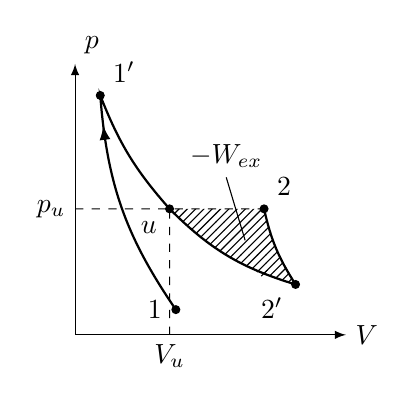
\begin{tikzpicture}[
	scale=0.8, every node/.style={scale=1},
  > = latex,
  dot/.style = {draw,fill,circle,inner sep=1pt},
  arrow inside/.style = {postaction=decorate,decoration={markings,mark=at position .55 with \arrow{>}}}
  ]
  \draw[<->] (0,4.3) node[above right] {$p$} |- (4.3,0) node[right] {$V$};
	\coordinate (a) at (1.6,0.4);
	\coordinate (b) at (0.4,3.8);

	\coordinate (c) at (3,2);
	\coordinate (d) at (3.5,0.8);

	\coordinate (u) at (1.5,2);
	\node[dot,label={below left:$u$}] at (u) {};

	\node[dot,label={left:$1$}] at (a) {};
	\node[dot,label={above right:$1'$}] at (b) {};

	\draw[thick, arrow inside] (a) to[bend left=15] (b) to[bend right=10] (u);

	\node[dot,label={above right:$2$}] at (c) {};
	\node[dot,label={below left:$2'$}] at (d) {};

	\draw[thick, arrow inside, pattern=north east lines] (c) to[bend right=10] (d) to[bend left=14] (u);
	\draw (2.7,1.5) to (2.4,2.5) node[above] {$-W_{ex}$};

  	\draw[dashed,thin] (0,2) node[left] {$p_u$} -- (c);
  	\draw[dashed,thin] (1.5,0) node[below] {$V_u$} -- (u);
\end{tikzpicture}
\end{multicols}

\begin{align*}
	-W_{ex} &= dh - TdS 
\end{align*}
\begin{multline*}
	-\dot{W}_{ex} = - (\dot{W}_t)_{rev} = -\frac{d}{dt} \left( U + m\left ( \frac{c^2}{2}+ gz \right) + p_uV - T_uS \right) \\  +  \sum_{j=1}^{K} \left(\dot{m}_j \left(h + \frac{c^2}{2} + gz -T_s \right) \right) + \sum_{l=1}^{K} \left( 1 - \frac{T_u}{T}\right) \dot{Q}_l 
\end{multline*}


Die Exergie der Enthalpie (offenes, stationäres System)
\begin{equation*}
	-\dot{W}_{ex,1u} = \dot{m}(h_1 - h_u -T_u(s_1 - s_u))
\end{equation*}
Die Exergie der inneren Energie (geschlossenes, instationäres System)
\begin{align*}
	- \dot{W}_{ex} &= - \frac{d}{dt}(U + p_uV -T_uS) \\
	-\dot{W}_{ex,1u} &= U_1 - U_u -p_u(V_1 - V_u) - T_u(S_1 - S_u) \\
	-\dot{W}_{ex,1u} &= H_1 + (p_1-p_u)V_1 - H_u- T_u(S_1 - S_u)
\end{align*}
Für Ideales Gas \\
\begin{align*}
	-W_{ex} &= mc_v(T_1 -T_u) + p_u(V_1 - V_u) - T_um \left(c_p \ln \left(\frac{T_1}{T_u}\right) -R_i \ln \left(\frac{p_1}{p_u}\right)\right) \\
	-W_{ex} &= m \left[c_p(T_1 - T_u) -T_u c_p \ln \left(\frac{T_1}{T_u}\right)\right] \leftarrow \text{isobar}
\end{align*}
Dampf/Luftdruckkammer
\begin{equation*}
	-W_{ex,1u} = m_1 [ u_1 - u_u + p_u ( v_1 - v_u) - T_u(s_1 - s_u)]
\end{equation*}
Die Exergie der Wärme (geschlossenes, stationäres System)
\begin{equation*}
	- \dot{W}_{ex} = \left(1 - \frac{T_u}{T_1} \right) \dot{Q}_1 = \eta_{th,C} \dot{Q}_1 \\
\end{equation*}

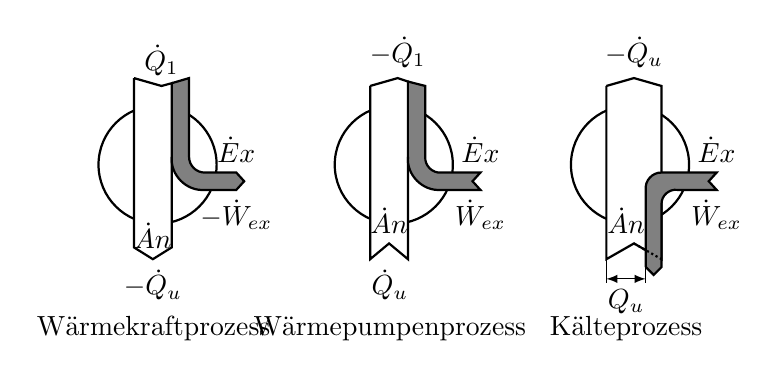
\begin{tikzpicture}[
		\thicc,
		scale=1, every node/.style={scale=1},
  		> = latex,
  		dot/.style = {draw,fill,circle,inner sep=1pt},
  		arrow inside/.style = {postaction=decorate,decoration={markings,mark=at position .55 with \arrow{>}}}
		]

	\draw 	(1,1.2) node [minimum size=1.5cm,circle,draw] {};

	\coordinate (a1) at (0.7,2.3);
	\coordinate (a2) at (1.05,2.2);
	\coordinate (a3) at (1.18,2.235);
	\coordinate (a4) at (1.18,0.15);
	\coordinate (a5) at (0.94,0);
	\coordinate (a6) at (0.7,0.15);
	\coordinate (a7) at (1.4,2.3);
	\coordinate (a8) at (1.4,1.3);
	\coordinate (a9) at (1.6,1.1);
	\coordinate (a10) at (2,1.1);
	\coordinate (a11) at (2.1,0.99);
	\coordinate (a12) at (2,0.88);
	\coordinate (a13) at (1.6,0.88);
	\coordinate (a14) at (1.18,1.3);
	
	\draw[fill=white] 	(a1) to (a2) to (a3) to (a4) to (a5) to (a6) to (a1);
	\draw[fill=gray] 	(a3) to (a7) to (a8) to[bend right=45] (a9) to (a10) to (a11) to (a12) to (a13) to[bend left=50] (a14);
	\draw (a3) to (a4);

	\draw 	(a2) node[above] {$\dot{Q}_1$};
	\draw 	(a5) node[above] {$\dot{A}n$};
	\draw 	(a5) node[below] {$-\dot{Q}_u$};
	\draw 	(a10) node[above] {$\dot{E}x$};
	\draw 	(a12) node[below] {$-\dot{W}_{ex}$};

	\draw (0.95,-0.6) node[below] {Wärmekraftprozess};


	\draw 	(4,1.2) node [minimum size=1.5cm,circle,draw] {};

	\coordinate (b1) at (3.7,2.2);
	\coordinate (b2) at (4.05,2.3);
	\coordinate (b3) at (4.18,2.256);
	\coordinate (b4) at (4.18,0);
	\coordinate (b5) at (3.94,0.2);
	\coordinate (b6) at (3.7,0.0);
	\coordinate (b7) at (4.4,2.2);
	\coordinate (b8) at (4.4,1.3);
	\coordinate (b9) at (4.6,1.1);
	\coordinate (b10) at (5.1,1.1);
	\coordinate (b11) at (5,0.99);
	\coordinate (b12) at (5.1,0.88);
	\coordinate (b13) at (4.6,0.88);
	\coordinate (b14) at (4.18,1.3);

	\draw[fill=white] 	(b1) to (b2) to (b3) to (b4) to (b5) to (b6) to (b1);
	\draw[fill=gray] 	(b3) to (b7) to (b8) to[bend right=50] (b9) to (b10) to (b11) to (b12) to (b13) to[bend left=50] (b14);
	\draw (b3) to (b4);

	\draw 	(b2) node[above] {$-\dot{Q}_1$};
	\draw 	(b5) node[above] {$\dot{A}n$};
	\draw 	(3.95,0) node[below] {$\dot{Q}_u$};
	\draw 	(b10) node[above] {$\dot{E}x$};
	\draw 	(b12) node[below] {$\dot{W}_{ex}$};

	\draw (3.95,-0.6) node[below] {Wärmepumpenprozess};


	\draw 	(7,1.2) node [minimum size=1.5cm,circle,draw] {};

	\coordinate (c1) at (6.7,2.2);
	\coordinate (c2) at (7.05,2.3);
	\coordinate (c3) at (7.4,2.2);
	\coordinate (c4) at (7.4,0);
	\coordinate (c5) at (7.05,0.2);
	\coordinate (c6) at (6.7,0.0);
	\coordinate (c7) at (7.2,-0.1);
	\coordinate (c8) at (7.2,0.88);
	\coordinate (c9) at (7.4,1.1);
	\coordinate (c10) at (8.1,1.1);
	\coordinate (c11) at (8,0.99);
	\coordinate (c12) at (8.1,0.88);
	\coordinate (c13) at (7.6,0.88);
	\coordinate (c14) at (7.4,0.70);
	\coordinate (c15) at (7.4,-0.1);
	\coordinate (c16) at (7.3,-0.2);

	\draw[fill=white] 	(c1) to (c2) to (c3) to (c4) to (c5) to (c6) to (c1);
	\draw[fill=gray] 	(c8)  to (c7)  to (c8)  to[bend left=50] (c9)  to (c10)  to (c11)  to (c12)  to (c13)  to[bend right=50] (c14)  to (c15) to (c16) to (c7);

	\draw 	(c2) node[above] {$-\dot{Q}_u$};
	\draw 	(6.95,0.2) node[above] {$\dot{A}n$};
	\draw 	(c10) node[above] {$\dot{E}x$};
	\draw 	(c12) node[below] {$\dot{W}_{ex}$};
	\draw[densely dotted] (c5) to (c4);
	\draw[thin] (c6) to (6.7,-0.3);
	\draw[thin] (c7) to (7.2,-0.3);
	\draw[thin,<->] (6.7,-0.25) to (7.2,-0.25);
	\draw (6.95,-0.25) node[below] {$Q_u$};

	\draw (6.95,-0.6) node[below] {Kälteprozess};
\end{tikzpicture}

                   
% _       __ /\// /|___/|                   __                           _ __   /\// /|___/|_ 
%| |     / ///\/ | __  /________ ___  ___  / /______ _____  ____ _____  (_) /__//\/ | __  / /_
%| | /| / / _ | / /_/ / ___/ __ `__ \/ _ \/ //_/ __ `/ __ \/ __ `/_  / / / __/ _ | / /_/ / __/
%| |/ |/ / __ |/___  / /  / / / / / /  __/ ,< / /_/ / /_/ / /_/ / / /_/ / /_/ __ |/___  / /_  
%|__/|__/_/ |_|/   |/_/  /_/ /_/ /_/\___/_/|_|\__,_/ .___/\__,_/ /___/_/\__/_/ |_|/   |/\__/  
%                                                 /_/                                         
\section{Wärmekapazität}

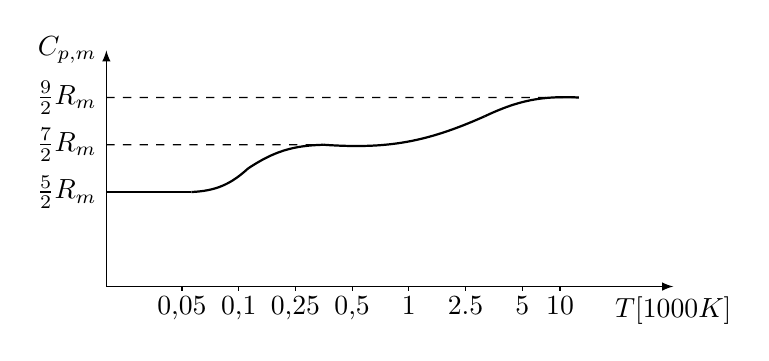
\begin{tikzpicture}[
	scale=1.2, every node/.style={scale=1},
  > = latex,
  dot/.style = {draw,fill,circle,inner sep=1pt},
  arrow inside/.style = {postaction=decorate,decoration={markings,mark=at position .55 with \arrow{>}}}
  ]
	\draw[<->] (0,2.5) node[left] {$C_{p,m}$} |- (6,0) node[below] {$T[1000K]$};

	\coordinate (a) at (0,1);
	\coordinate (b) at (0.9,1);
	\coordinate (c) at (1.5,1.25);
	\coordinate (d) at (2.3,1.5);
	\coordinate (e) at (4,1.8);
	\coordinate (f) at (5,2);
	
	\coordinate (g) at (0.8,0);
	\coordinate (h) at (1.4,0);
	\coordinate (i) at (2.0,0);
	\coordinate (j) at (2.6,0);
	\coordinate (k) at (3.2,0);
	\coordinate (l) at (3.8,0);
	\coordinate (m) at (4.4,0);
	\coordinate (n) at (4.8,0);

	\draw[dashed] (0,2) node[left] {$\frac{9}{2}R_m$} -- (f);
	\draw[dashed] (0,1.5) node[left] {$\frac{7}{2}R_m$} -- (d);
	\draw (a) node[left] {$\frac{5}{2}R_m$};

	\draw[thick] (a) to (b);
	\draw[thick] (b) to[bend right=20] (c);
	\draw[thick] (c) to[bend left=16] (d);
	\draw[thick] (d) to[bend right=14] (e);
	\draw[thick] (e) to[bend left=14] (f);

	\draw (g) node[below] {0,05} to ($ (g) - (0,0.05) $);
	\draw (h) node[below] {0,1} to ($ (h) - (0,0.05) $);
	\draw (i) node[below] {0,25} to ($ (i) - (0,0.05) $);
	\draw (j) node[below] {0,5} to ($ (j) - (0,0.05) $);
	\draw (k) node[below] {1} to ($ (k) - (0,0.05) $);
	\draw (l) node[below] {2.5} to ($ (l) - (0,0.05) $);
	\draw (m) node[below] {5} to ($ (m) - (0,0.05) $);
	\draw (n) node[below] {10} to ($ (n) - (0,0.05) $);
\end{tikzpicture}

\begin{align*}
	&	C_{v,m} = \frac{1}{\kappa - 1} R_m
		&&C_{p,m} = \frac{\kappa}{\kappa -1}R_m \\
	&	c_v = \frac{1}{\kappa - 1 }R_j 
		&&c_p = \frac{\kappa}{\kappa -1}R_j \\
	&	\kappa = \frac{c_p}{c_v}
	&&R = c_p - c_v \\
	&R = \frac{R_m}{M}
	&&R_m = 8,3143\left[\frac{kJ}{kmolK}\right] \\
	\end{align*}
	\begin{align*}
		C_{m,v} &= \frac{f}{2} R_m = \frac{f_{trans} + f_{rot} + f_{vib}}{2}R_m \\
		C_{m,p} &= \frac{f + 2}{2}R \\
		\kappa &= \frac{f + 2}{f} \\
		f_{trans} &= 3 \quad (\text{für die 3 Translatorischen Freiheitsgrade}) \\
		f_{rot} &\in \{0,2,3\} \quad \text{\{Einatomig, Linear, Verzweigt\}} \\
		\begin{tabular}{l}
		$ \quad	f_{vib} $\\
			 \\
			 \\
			 \\
		\end{tabular}
		&
		\begin{tabular}{llL{4cm}lll}
			$= 2 \cdot l$ &, $l = 1$  &Normalschwingungen der Atomkerne (Kann für komplexere Moleküle auch > 1 sein.)  &  &  & \\
		\end{tabular}
	\end{align*}

		
			%2 \cdot l,  \quad l &= \text{1,  Freiheitsgrade für Vibration} \\
%	\begin{multline*}
%		C_{v,m} = \underbrace{3 + \frac{R_m}{2}}_{\text{translatorisch}} + \underbrace{\frac{n_{\text{rot}}  R_m}{2}}_{\text{rotatorisch}}  
%		+ \underbrace{R_M ( 3n_{\text{Atome}} - 3 - n_{rot})}_{\text{vibratorisch}}  \\
%		+ \underbrace{C_{v,m,Elektronenanregung}}_{\text{Relevant ab: }T \approx 10^4K } 
%	\end{multline*}

%  ______          __          _           __       
% /_  __/__  _____/ /_  ____  (_)_________/ /_  ___ 
%  / / / _ \/ ___/ __ \/ __ \/ / ___/ ___/ __ \/ _ \
% / / /  __/ /__/ / / / / / / (__  ) /__/ / / /  __/
%/_/  \___/\___/_/ /_/_/ /_/_/____/\___/_/ /_/\___/ 
%                                                         
%    ___                                 __                 
%   /   |  ____ _      _____  ____  ____/ /_  ______  ____ _
%  / /| | / __ \ | /| / / _ \/ __ \/ __  / / / / __ \/ __ `/
% / ___ |/ / / / |/ |/ /  __/ / / / /_/ / /_/ / / / / /_/ / 
%/_/  |_/_/ /_/|__/|__/\___/_/ /_/\__,_/\__,_/_/ /_/\__, /  
%                                                  /____/   

\onecolumn
\section{Technische Anwendung}

\begin{centering}
\begin{tabular}{lll} 
	\begin{tabular}{l}
	adiabat \\ $(c_p = const.)$
	\end{tabular}
	&
 $ \displaystyle W_{t,12} = mc_p(T_2 - T_1) = \frac{\kappa}{\kappa -1}(p_2V_2 - p_1V_1)$ &
 $Q_{12}=0$\\ \hline
	\begin{tabular}{l}
	reversibel adiabat \\ 
	$ \kappa = const.$
	\end{tabular}
	&
 $\displaystyle W_{t,12} = \frac{\kappa}{\kappa -1} (p_1 V_1)\left[\left(\frac{p_2}{p_1}\right)^{\frac{\kappa - 1}{\kappa}} - 1 \right]$ &
 $\displaystyle Q_{12}=0$ \\ \hline
	\begin{tabular}{l}
	irreversibel adiabat \\ 
	als Polytrope \\ 
	$n>\kappa; n,\kappa = const.$
	\end{tabular}
	&
 $\displaystyle W_{t,12} = \frac{\kappa}{\kappa -1} (p_1 V_1)\left[\left(\frac{p_2}{p_1}\right)^{\frac{n - 1}{n}} - 1 \right]$ &
 $\displaystyle Q_{12}=0$ \\ \hline
	\begin{tabular}{l}
	reversibel polytrop \\ $n,\kappa = const.$ 
	\end{tabular}
		&
 $\displaystyle W_{t,12} = \frac{n}{n-1}(p_2V_2 - p_1V_1)$ &
 $\displaystyle Q_{12} = mc_n(T_2-T_1)$ \\
	 &
 $\displaystyle \qquad \: = \frac{n}{n-1}mR(T_2-T_1)$ &
  $\displaystyle \quad \;\;\; =\frac{n-\kappa}{(n-1)(\kappa-1)}(p_1V_1) \left[ \left( \frac{p_2}{p_1}\right)^{\frac{n-1}{n} - 1}\right]$ \\
	 &
 $\displaystyle \qquad \: = \frac{n}{n-1}(p_1V_1) \left[\left( \frac{p_2}{p_1}\right)^{\frac{n-1}{n}} - 1 \right]$ &
 $ \displaystyle c_n \;\; = \frac{n-\kappa}{n-1}cv$\\ \hline
	 isotherm &
 $ \displaystyle  W_{t,12} = (p_1V_1) \ln \left(\frac{p_2}{p_1}\right)$ &
 $ \displaystyle Q_{12} = -W_{t,12}$ \\
\end{tabular}

\end{centering}
\bigskip

\begin{tabular}{lllll}
	Thermischer Wirkungsgrad 
	&
	$\eta_{th}$ & $\displaystyle = \frac{-w}{q_{zu}} = \frac{\text{Nutzen}}{\text{Aufwand}}$ &$= \displaystyle 1 - \frac{|q_{ab}|}{q_{zu}}$ &
	\multirow{2}{*}{
	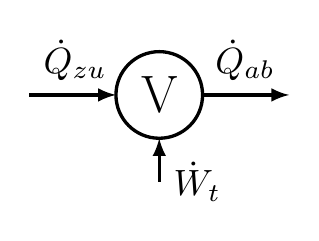
\begin{tikzpicture}
		[remember picture, 
		very thick,
		scale=1, every node/.style={scale=1.1},
  		> = latex,
  		dot/.style = {draw,fill,circle,inner sep=1pt},
  		arrow inside/.style = {postaction=decorate,decoration={markings,mark=at position .55 with \arrow{>}}}
		]
		\pic (B) {verdichter};
	\end{tikzpicture}}
	\\\\
	Isentroper Verdichterwirkungsgrad
	& 
	$\eta_{sV}$ & $\displaystyle = \frac{w_{t,12,rev}}{w_{t,12}} =\frac{h_{2,rev} - h_1}{h_2 - h_1}$ &  $ \displaystyle = \underbrace{\frac{T_{2,rev} -T_1}{T_2 -T_1}}_{}$ \\
	&&& $\quad$ideales Gas \\
	Isentroper  Turbinenwirkungsgrad 
	&
	$\eta_{sT}$ & $\displaystyle = \frac{w_{t,12}}{W_{t,12,rev}} = \frac{h_1 - h_2}{h_1 - h_{2,rev}}$ & $ \displaystyle = \overbrace{\frac{T_1 -T_2}{T_1 -T_{2,rev}}}^{\text{}}$ &
	\multirow{2}{*}{
	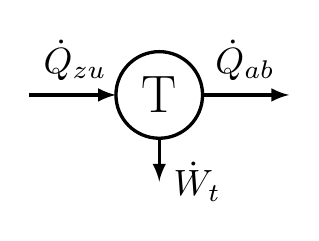
\begin{tikzpicture}
		[remember picture,
		very thick,
		scale=1, every node/.style={scale=1.1},
  		> = latex,
  		dot/.style = {draw,fill,circle,inner sep=1pt},
  		arrow inside/.style = {postaction=decorate,decoration={markings,mark=at position .55 with \arrow{>}}}
		]
		\pic (A) {turbine};
	\end{tikzpicture}}
	\\\\
	Dampfkraftprozess Wirkungsgrad 
	&
	$n_{th}$ &$\displaystyle = 1 - \frac{|q_{61}|}{q_{23}+q_{34} + q_{45}}$ 
	& 
	$\displaystyle = 1 - \frac{h_6 - h_1}{h_5 -  h_2}$ \\\\
	Leistungszahl Kältemaschine &
	$\epsilon_{K(A)}$ &$\displaystyle = \frac{q_{zu}}{w} = \frac{\dot{Q}_0}{\dot{W}}$ & 
%	\multirow{2}{*}{
%	\begin{tikzpicture}
%		[remember picture,
%		very thick
%		]
%		\pic (C) {kaelteprozess};
%	\end{tikzpicture}}
	\\\\
	Leistungszahl Kaltdampfprozess &
	$\epsilon_K$ & $\displaystyle = \frac{q_0}{|q| - q_0} = \frac{q_o}{w_t}$ &$\displaystyle = \frac{h_1 - h_6}{h_2 - h_1}$ 
	\\\\
	Linkslaufender Carnotprozess &
	$\epsilon_{carnot}$ &$\displaystyle = \frac{T_k}{T_H-T_K}$ \\
	Leistungszahl Wärmepumpe &
	$\epsilon_{WP}$ & $\displaystyle = \frac{q}{|q| - q_0} = \frac{|q|}{w_t} = \frac{q_{ab}}{w}$ &$\displaystyle = \frac{h_2 - h_5}{h_2 - h_1} = 1 + \epsilon_{K(A)}$ \\\\
	Kälteleistung Wärmepumpe &
	$\dot{Q}_0$ &$\displaystyle= \dot{m}(h_2 - h_5)$ \\\\
	Leistungszahl Kaltluftprozess &
	$\epsilon_{K}$ &$\displaystyle = \frac{1}{\left(\frac{p}{p_0}\right)^{\frac{\kappa - 1}{\kappa} - 1}}$ \\\\
	Kälteleistung Kaltluftprozess &
	$\dot{Q}_0$ &$\displaystyle= \dot{m}(h_1 - h_6)$ \\\\
	Arbeit der Enthalpie &
	$W_t=Q$ & $\displaystyle = mdh = mcpdT$ \\\\
	Verdichtungsverhältnis &
	$\epsilon$ &$= v_1/v_2$ \\
	Drucksteigerungsverhältniss &
	$\psi$ &$ = p_3/p_2$ \\
	Einspritzverhältniss &
	$\varphi $ &$= v_4/v_3$ \\
	Temperaturverhältnis &
	$\tau$ &$ =T_3/T_1$ \\
	Verdrichtungsdruckverhältnis &
	$\pi$ = & $ = p_2/p_1$ \\
	für Joule-Prozess &
	$\pi_{opt}$ & $ \displaystyle = \tau^{\frac{\kappa}{2(\kappa -1)}}$ \\
	
	
\end{tabular}

\pagebreak

\begin{multicols}{2}
\section{Kolbenverdichter}

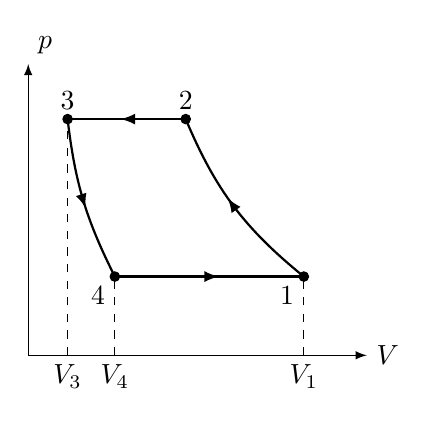
\begin{tikzpicture}
	[
	%\thicc,
  	> = latex,
  	dot/.style = {draw,fill,circle,inner sep=1pt},
  	arrow inside/.style = {postaction=decorate,decoration={markings,mark=at position .55 with \arrow{>}}}
  	]

  	\draw[<->] (0,3.7) node[above right] {$p$} |- (4.3,0) node[right] {$V$};

  	\coordinate (@1) at (3.5,1);
  	\coordinate (@2) at (2,3);
  	\coordinate (@3) at (0.5,3);
  	\coordinate (@4) at (1.1,1);

	\draw[fill] (@1) circle (0.06) node[below left] {1};
	\draw[fill] (@2) circle (0.06) node[above] {2};
	\draw[fill] (@3) circle (0.06) node[above] {3};
	\draw[fill] (@4) circle (0.06) node[below left] {4};
	

	\draw[thick, arrow inside] (@1) to[bend left=14] (@2);
 	\draw[thick, arrow inside] (@2) to (@3);
	\draw[thick, arrow inside] (@3) to[bend right=10] (@4);
 	\draw[thick, arrow inside] (@4) to (@1);
	
  	\draw[dashed,thin] (3.5,0) node[below] {$V_1$} -- (@1);
  	\draw[dashed,thin] (0.5,0) node[below] {$V_3$} -- (@3);
  	\draw[dashed,thin] (1.1,0) node[below] {$V_4$} -- (@4);
	
%	\draw (5,3.0) node[right] {$V1 =$ Maximales Zylindervolumen};
%	\draw (5,2.2) node[right] {$V2 =$ Volumen nach Verdichtung};
%	\draw (5,1.4) node[right] {$V3 =$ };
%	\draw (5,0.6) node[right] {$V4 =$ Schädlicher Raum};
	
\end{tikzpicture}


\begin{alignat*}{2}
	\small
	\mu &= \frac{V_1 - V_4}{V_1-V3}, \qquad \epsilon_S = \frac{V_3}{V_1 - V_3},  \quad 
	\mu = 1 - \epsilon_S \left[\left(\frac{p_2}{p_1}\right)^{\frac{1}{n}} -1 \right] \\
W_t	&= \frac{n}{n-1}p_1(V_1-V_4) \left[\left(\frac{p_2}{p_1}\right)^{\frac{n-1}{n}} - \right] \\
\end{alignat*}

	\section{Strahltriebwerk}
	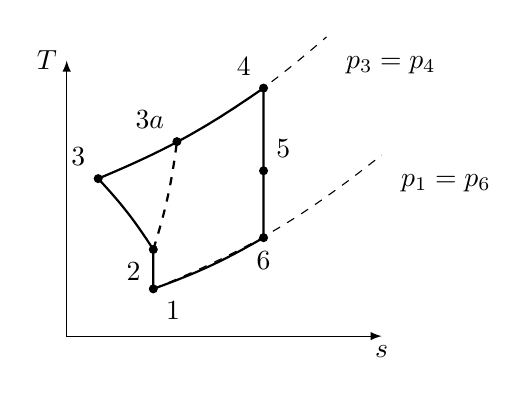
\begin{tikzpicture}
	[
	%\thicc,
  	> = latex,
  	dot/.style = {draw,fill,circle,inner sep=1pt},
  	arrow inside/.style = {postaction=decorate,decoration={markings,mark=at position .55 with \arrow{>}}}
  	]
		\draw[<->] (0,4) node[left] {$T$} |- (4,0.5) node[below] {$s$};

		\coordinate (a) at (1.1,1.1);
		\coordinate (b) at (4,2.8);
		\coordinate (c) at (0.4,2.5);
		\coordinate (d) at (3.3,4.3);
		\coordinate (@1) at (1.1,1.1);
		\coordinate (@2) at (1.1,1.6);
		\coordinate (@3) at (0.4,2.5);
		\coordinate (@3a) at (1.4,2.97);
		\coordinate (@4) at (2.5,3.65);
		\coordinate (@5) at (2.5,2.6);
		\coordinate (@6) at (2.5,1.75);

		\node[dot,label={below right:$1$}] at (@1) {};
		\node[dot,label={below  left:$2$}] at (@2) {};
		\node[dot,label={above  left:$3$}] at (@3) {};
		\node[dot,label={above  left:$3a$}] at (@3a) {};
		\node[dot,label={above  left:$4$}] at (@4) {};
		\node[dot,label={above right:$5$}] at (@5) {};
		\node[dot,label={below      :$6$}] at (@6) {};
	
		\node[label={below right:$p_3 = p_4$}] at (d) {};
		\node[label={below right:$p_1 = p_6$}] at (b) {};

		\draw[dashed] (a) to[bend right=8] (b);
		\draw[dashed] (c) to[bend right=9] (d);

		\draw[thick] (@1) to (@2) to[bend right=5] (@3) to[bend right=6] (@4) to (@5) to (@6) to[bend left=5] (@1);
		\draw[thick, dashed] (@2) to[bend right=5] (@3a);
		
	\end{tikzpicture}
	\begin{align*}
		\text{Anström}&\text{geschwindigkeit: } \\ 
		\frac{1}{2} c^2_1 &= c_p (T_2 - T_1) \\
		w_{2-3} &= - w_{4-5} = c_p(T_3-T_2) \\
		\Delta E_{kin} &= dH \\
	\end{align*}

\end{multicols}


\begin{multicols}{2}
%  ______           __                             ___      __    __           
% /_  __/_  _______/ /_  ____ _   _____  _________/ (_)____/ /_  / /____  _____
%  / / / / / / ___/ __ \/ __ \ | / / _ \/ ___/ __  / / ___/ __ \/ __/ _ \/ ___/
% / / / /_/ / /  / /_/ / /_/ / |/ /  __/ /  / /_/ / / /__/ / / / /_/  __/ /    
%/_/  \__,_/_/  /_.___/\____/|___/\___/_/   \__,_/_/\___/_/ /_/\__/\___/_/     
%                                                                              
\section{Turboverdichter}

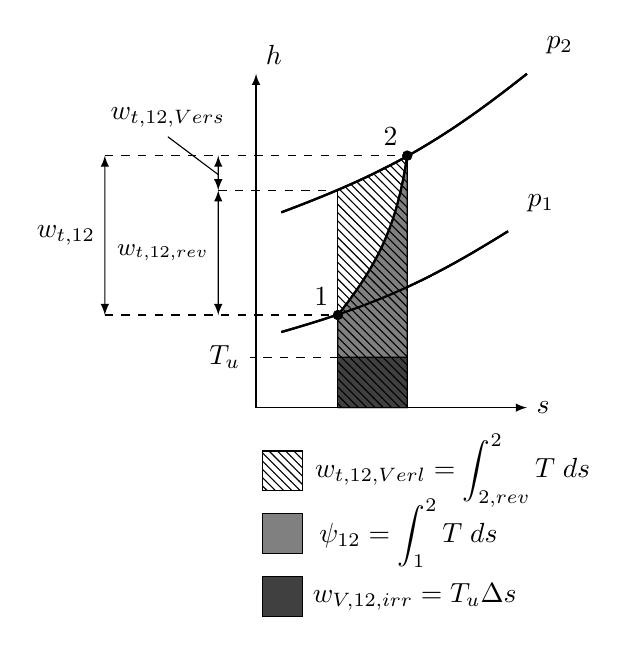
\begin{tikzpicture}[
	scale=0.8, every node/.style={scale=1},
  > = latex,
  dot/.style = {draw,fill,circle,inner sep=1pt},
  arrow inside/.style = {postaction=decorate,decoration={markings,mark=at position .55 with \arrow{>}}}
  ]
  	\draw[<->] (0,5.3) node[above right] {$h$} |- (4.3,0) node[right] {$s$};

	\coordinate (@1) at (0.4,1.2);
	\coordinate (@2) at (4,2.8);
	\coordinate (@3) at (0.4,3.1);
	\coordinate (@4) at (4.3,5.3);
	\coordinate (@5) at (1.3,0);
	\coordinate (@6) at (1.3,3.45);
	\coordinate (@7) at (-0.6,3.45);
	\coordinate (@8) at (-2.4,1.470);
	\coordinate (@9) at (1.3,1.470);
	\coordinate (@10) at (-2.4,4);
	\coordinate (@11) at (2.4,4);
	\coordinate (@12) at (2.4,0);

	\node[label={above right:$p_1$}] at (@2) {};
	\node[label={above right:$p_2$}] at (@4) {};

	\draw[thick] (@1) to[bend right=8] (@2);
	\draw[thick] (@3) to[bend right=9] (@4);
	\draw[thick] (@9) node[dot] {} to[bend right=15] (@11) node[dot] {};
	\draw[fill=gray] (@9) to (@5) to (@12) to (@11) to[bend left=15] (@9);
	\draw[fill=darkgray] (@5) to (@12) to (2.4,0.8) to (1.3,0.8);
	\draw[pattern=north west lines] (@6) to (@5) to (@12) to (@11);
	\draw[dashed] (@5) to (@6);
	\draw[dashed] (@7) to (@6);
	\draw[dashed] (@8) to (@9);
	\draw[dashed] (@10) to (@11);
	\draw[dashed] (@11) to (@12);
	\draw[dashed] (1.3,0.8) to (-0.1,0.8) node[left] {$T_u$};

	\draw (@9) node[above left] {1};
	\draw (@11) node[above left] {2};

	\draw[<->] (-0.6,1.47) to node[midway, left] {\small $w_{t,12,rev}$} (@7);
	\draw[<->] (-0.6,4) to  (@7);
	\draw[<->] (-2.4,1.47) to node[midway, left] {$w_{t,12}$} (@10);
	\draw[thin] (-1.4,4.3) node[above] {$w_{t,12,Vers}$} to (-0.6,3.7);

	\draw[thick] (@1) to[bend right=8] (@2);
	\draw[thick] (@3) to[bend right=9] (@4);
	\draw[thick] (@9) node[dot] {} to[bend right=15] (@11) node[dot] {};

	\draw (0.42,-1) node[pattern=north west lines, minimum size=5mm,draw] {};
	\draw (3.12,-1) node {$\displaystyle w_{t,12,Verl} = \int_{2,rev}^{2} T\; ds$};
	\draw (0.42,-2) node[fill=gray, minimum size=5mm,draw] {};
	\draw (2.42,-2) node {$\displaystyle \psi_{12} = \int_{1}^{2} T\; ds$};
	\draw (0.42,-3) node[fill=darkgray, minimum size=5mm,draw] {};
	\draw (2.52,-3) node {$\displaystyle w_{V,12,irr} = T_u\Delta s$};

\end{tikzpicture}
\\

\section{Clausius-Rankine-Prozess}

\begin{tikzpicture}[
	scale=1, every node/.style={scale=1},
  > = latex,
  dot/.style = {draw,fill,circle,inner sep=1pt},
  arrow inside/.style = {postaction=decorate,decoration={markings,mark=at position .55 with \arrow{>}}}
  ]
  	\draw[<->] (0,4) node[above right] {$T$} |- (5,0) node[right] {$s$};
	
	\coordinate (@1) at (0.6,0.8);
	\coordinate (@2) at (0.6,1.4);
	\coordinate (@3) at (1.4,2.5);
	\coordinate (@3a) at (1.4,0.8);
	\coordinate (@4) at (3.4,2.5);
	\coordinate (@4a) at (3.4,0.8);
	\coordinate (@5) at (3.8,3.7);
	\coordinate (@6) at (3.8,0.8);
	\coordinate (@6a) at (3.8,2.5);
	\coordinate (@7) at (4.3,3.7);
	\coordinate (@8) at (4.3,0.8);
	\coordinate (k) at (2.4,3.2);

	\draw[arrow inside, thick] (@1) to (@2);
	\draw[arrow inside, thick] (@2) to[bend right=10] (@3);
	\draw[arrow inside, thick] (@3) to (@4);
	\draw[arrow inside, thick] (@4) to[bend right=10] (@5);
	\draw[arrow inside, thick] (@5) to (@6);
	\draw[arrow inside, thick] (@6) to (@1);

	\draw[arrow inside, thick, dotted] (@6a) to (@7);
	\draw[arrow inside, thick, dotted] (@7) to (@8);
	\draw[arrow inside, thick, dotted] (@8) to (@6);

	\draw (0.3,0.7) to[bend right=10] (@3);
	\draw (@3) parabola bend (k) (@4);
	\draw (@4) to[bend right=10] (4.8,0.2);

	\draw[dashed] (@3) to (@4) to (@4a) to (@3a) to (@3);
	\draw (k) node[above] {K};
	\draw[dashed] (-0.1,3.7) node[left] {$T_{max}$} to (4.9,3.7);

	\node[dot,label={below right:$1$}] at (@1) {};
	\node[dot,label={below  left:$2$}] at (@2) {};
	\node[dot,label={above  left:$3$}] at (@3) {};
	\node[dot,label={below  left:$4$}] at (@4) {};
	\node[dot,label={above right:$5$}] at (@5) {};
	\node[dot,label={below      :$6$}] at (@6) {};
	\node[dot,label={below right:   }] at (@6a){};
	\node[dot,label={above right:$7$}] at (@7) {};
	\node[dot,label={      right:$8$}] at (@8) {};

	\draw (0.6,2.3) node[above] {\tiny $p =$ const.} to (0.8,1.583); 
	\draw (3.3,3.3) node[above] {\tiny $p =$ const.} to (3.72,3.2); 
	\draw (2.6,1.5) node[above] {\small $p,T =$ const.} to (3.2,0.8); 
	\draw (1.6,2.5) to (2,2.1); 

	\draw[thick] (0,-0.3) to (1,-0.3) node[right] {\small Clausius-Rankine Prozess};
	\draw[thick, dotted] (0,-0.7) to (1,-0.7) node[right] {\small mit Zwischenüberhitzung};
	\draw[dashed] (0,-1.1) to (1,-1.1) node[right] {\small Carnot Prozess};
	\draw (-0.2,-1.9) node[right] {$\displaystyle \eta_{th} = 1 - \frac{|q_{61}|}{q_{23} + q_{34} + q_{45}} = 1- \frac{h_6 - h_1}{h_5 -h_2}$};
	\draw (-0.2,-2.9) node[right] {$\displaystyle \eta_{th,ZÜ} = 1 - \frac{|q_{81}|}{q_{23} + q_{34} + q_{45} + q_{67}} $};
	\draw (-0.2,-3.9) node[right] {$\displaystyle \eta_{th,ZÜ} = 1- \frac{h_8 - h_1}{h_5 -h_2 + h_7 - h_6}$};
\end{tikzpicture}

\end{multicols}



\section{Kaltdampfprozess}
\begin{multicols}{2}

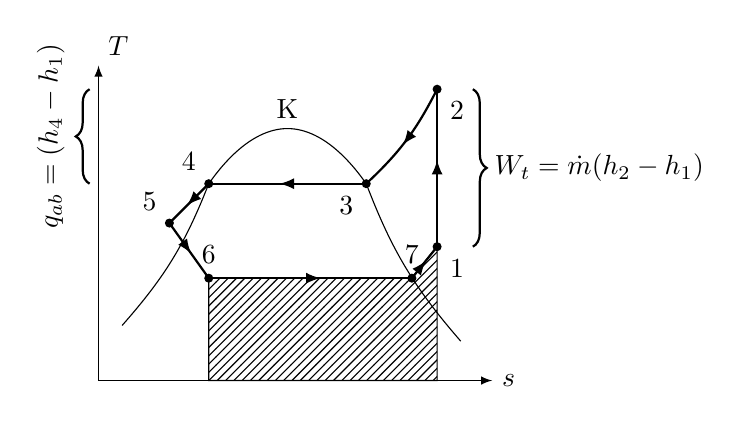
\begin{tikzpicture}[
	scale=1, every node/.style={scale=1},
  > = latex,
  dot/.style = {draw,fill,circle,inner sep=1pt},
  arrow inside/.style = {postaction=decorate,decoration={markings,mark=at position .55 with \arrow{>}}}
  ]
  	\draw[<->] (0,4) node[above right] {$T$} |- (5,0) node[right] {$s$};
	
	\coordinate (@7) at (3.98,1.3);
	\coordinate (@6) at (1.4,1.3);
	\coordinate (@5) at (0.9,2);
	\coordinate (@4) at (1.4,2.5);
	\coordinate (@3) at (3.4,2.5);
	\coordinate (@2) at (4.3,3.7);
	\coordinate (@1) at (4.3,1.7);
	\coordinate (k) at (2.4,3.2);

	\draw[arrow inside, thick] (@1) to (@2);
	\draw[arrow inside, thick] (@2) to[bend left=10] (@3);
	\draw[arrow inside, thick] (@3) to (@4);
	\draw[arrow inside, thick] (@4) to (@5);
	\draw[arrow inside, thick] (@5) to (@6);
	\draw[arrow inside, thick] (@6) to (@7);
	\draw[arrow inside, thick] (@7) to (@1);

	\draw (0.3,0.7) to[bend right=10] (@4);
	\draw (@3) parabola bend (k) (@4);
	\draw (@3) to[bend right=10] (4.6,0.5);

	\draw (k) node[above] {K};

	\node[dot,label={below right:$1$}] at (@1) {};
	\node[dot,label={below right:$2$}] at (@2) {};
	\node[dot,label={below  left:$3$}] at (@3) {};
	\node[dot,label={above  left:$4$}] at (@4) {};
	\node[dot,label={above  left:$5$}] at (@5) {};
	\node[dot,label={above      :$6$}] at (@6) {};
	\node[dot,label={above      :$7$}] at (@7) {};

	\draw[pattern=north east lines] (@1) to (@7) to (@6) to (1.4,0) to (4.3,0) to (@1);

	\draw[thick] [decorate, decoration={brace, amplitude=5pt, mirror, raise=3ex}] (@1) to node[right=6mm] {$W_t = \dot{m}(h_2 - h_1)$} (@2);
	\draw[thick] [decorate, decoration={brace, amplitude=5pt,mirror, raise=10ex}] ($(@2)-(2.9,0)$) to node[sloped,above=17mm] {$q_{ab} = (h_4 - h_1)$} (@4);

\end{tikzpicture}

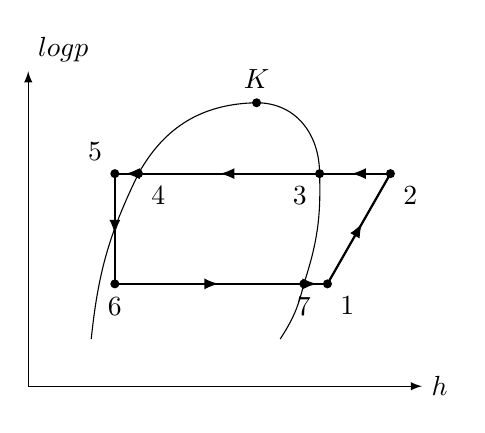
\begin{tikzpicture}
	[
	scale=1, every node/.style={scale=1},
  > = latex,
  dot/.style = {draw,fill,circle,inner sep=1pt},
  arrow inside/.style = {postaction=decorate,decoration={markings,mark=at position .55 with \arrow{>}}}
  ]
	\draw[<->] (0,4) node[above right] {$log p$} |- (5,0) node[right] {$h$};
	
	\coordinate (@7) at (3.5,1.3);
	\coordinate (@6) at (1.1,1.3);
	\coordinate (@5) at (1.1,2.7);
	\coordinate (@4) at (1.4,2.7);
	\coordinate (@3) at (3.7,2.7);
	\coordinate (@2) at (4.6,2.7);
	\coordinate (@1) at (3.8,1.3);
	\coordinate (k) at (2.9,3.6);

	\draw[arrow inside, thick] (@1) to (@2);
	\draw[arrow inside, thick] (@2) to (@3);
	\draw[arrow inside, thick] (@3) to (@4);
	\draw[arrow inside, thick] (@4) to (@5);
	\draw[arrow inside, thick] (@5) to (@6);
	\draw[arrow inside, thick] (@6) to (@7);
	\draw[arrow inside, thick] (@7) to (@1);

	\draw (k) to[bend right=30] (@4);
	\draw (k)  .. controls (3.4,3.6) and (3.7,3.2) .. (@3);
	\draw (@3) to[bend left=10] (@7);
	\draw (@7) to[bend left=10] (3.2,0.6);
	\draw (@4) to[bend right=10] (0.8,0.6);

	sheesh
	\node[dot,label={below right:$1$}] at (@1) {};
	\node[dot,label={below right:$2$}] at (@2) {};
	\node[dot,label={below  left:$3$}] at (@3) {};
	\node[dot,label={below right:$4$}] at (@4) {};
	\node[dot,label={above  left:$5$}] at (@5) {};
	\node[dot,label={below      :$6$}] at (@6) {};
	\node[dot,label={below      :$7$}] at (@7) {};
	\node[dot,label={above      :$K$}] at (k) {};

	%\draw[pattern=north east lines] (@1) to (@7) to (@6) to (1.4,0) to (4.3,0) to (@1);

\end{tikzpicture}

\end{multicols}

\pagebreak
\begin{multicols}{2}

%    __    _           __   
%   / /   (_)___  ____/ /__ 
%  / /   / / __ \/ __  / _ \
% / /___/ / / / / /_/ /  __/
%/_____/_/_/ /_/\__,_/\___/ 
%                           
\section{Luftverflüssigung nach Linde}
	

	\begin{tikzpicture}
	[
	scale=1, every node/.style={scale=1},
  > = latex,
  dot/.style = {draw,fill,circle,inner sep=1pt},
  arrow inside/.style = {postaction=decorate,decoration={markings,mark=at position .55 with \arrow{>}}}
  ]
	\draw[<->] (-.3,5) node[above right] {$T$} |- (4,0) node[right] {$s$};

	\coordinate (1) at (4,4);
	\coordinate (2) at (2.5,4);
	\coordinate (3) at (0.7,1.5);
	\coordinate (4a) at (0.3,0.8);
	\coordinate (4) at (1.1,0.8);
	\coordinate (4b) at (1.8,0.8);
	\coordinate (5) at (3.9,3.8);
	\coordinate (p1) at (4.4,5);
	\coordinate (p2) at (2.9,5);
	\draw[dashed] (p1) node[right] {$p_1$} to[bend left=8] (1);
	\draw[dashed] (p2) node[right] {$p_2$} to[bend left=8] (2);

		\draw[thick] (1) to (2) to[bend left=8] (3) to[bend left=39] (4) to (4b) to[bend right=8] (5) to (1);
		\draw[thick] (4) to (4a);

		\draw (4a) to (0.3,0);
		\draw (4) to (1.1,.4);
		\draw (4b) to (1.8,0);

		\draw[<->] (0.3,0.4) to node[above, scale=0.9] {x} (1.1,0.4);
		\draw[<->] (1.8,0.4) to node[above, scale=0.9] {1-x} (1.1,0.4);

		\draw[dashed] (4a) parabola bend ($(4)+(0,0.7)$) (4b);
		
		\draw (-2.96,0) node {};

	\node[dot,label={right:$1$}] at (1) {};
	\node[dot,label={above left:$2$}] at (2) {};
	\node[dot,label={above  left:$3$}] at (3) {};
	\node[dot,label={left:$4'$}] at (4a) {};
	\node[dot,label={above right:$4$}] at (4) {};
	\node[dot,label={right:$4''$}] at (4b) {};
	\node[dot,label={below  right:$5$}] at (5) {};
	\node[dot,label={above:$\small K$}] at ($(4)+(0,0.7)$) {};
	\end{tikzpicture}

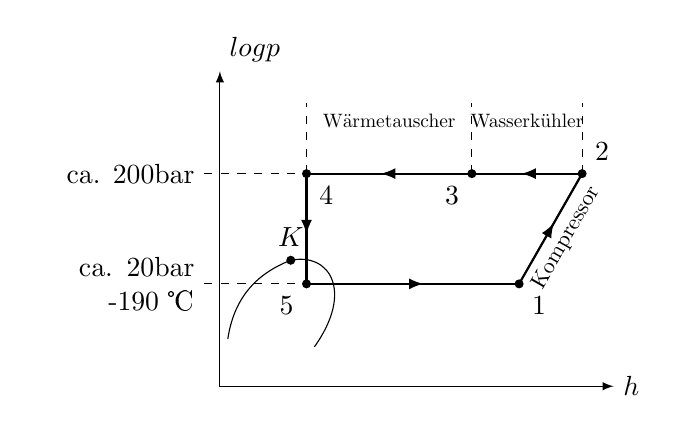
\begin{tikzpicture}[
	scale=1, every node/.style={scale=1},
  > = latex,
  dot/.style = {draw,fill,circle,inner sep=1pt},
  arrow inside/.style = {postaction=decorate,decoration={markings,mark=at position .55 with \arrow{>}}}
  ]
	\draw[<->] (0,4) node[above right] {$log p$} |- (5,0) node[right] {$h$};
	
	\coordinate (@1) at (3.8,1.3);
	\coordinate (@2) at (4.6,2.7);
	\coordinate (@3) at (3.2,2.7);
	\coordinate (@4) at (1.1,2.7);
	\coordinate (@5) at (1.1,1.3);
	\coordinate (k) at (0.9,1.6);

	\draw[arrow inside, thick] (@1) to node[below, sloped, scale=0.8] {Kompressor} (@2);
	\draw[arrow inside, thick] (@2) to node[above=5mm, scale=0.7] {Wasserkühler} (@3);
	\draw[arrow inside, thick] (@3) to node[above=5mm, scale=0.7] {Wärmetauscher} (@4);
	\draw[arrow inside, thick] (@4) to (@5);
	\draw[arrow inside, thick] (@5) to (@1);

	\draw (k) to[bend right=30] (0.1,0.6);
	\draw (k)  .. controls (1.4,1.7) and (1.7,1.2) .. (1.2,0.5);

	\node[dot,label={below right:$1$}] at (@1) {};
	\node[dot,label={above right:$2$}] at (@2) {};
	\node[dot,label={below  left:$3$}] at (@3) {};
	\node[dot,label={below right:$4$}] at (@4) {};
	\node[dot,label={below  left:$5$}] at (@5) {};
	\node[dot,label={above      :$K$}] at (k) {};

	\draw[dashed] (-0.2,2.7) node[left] {ca. 200bar} to (@4);
	\draw[dashed] (-0.2,1.3) node[left, text width=20mm, align=right] {ca. 20bar {-190 \textcelsius} } to (@5);
	\draw[dashed] (@4) to ($(@4)+(0,0.9)$);
	\draw[dashed] (@3) to ($(@3)+(0,0.9)$);
	\draw[dashed] (@2) to ($(@2)+(0,0.9)$);


\end{tikzpicture}

	\begin{align*}
		h_2 &= (q-x)h_{4'} + xh_5 \\
		(1-x) &= \frac{h_5 - h_2}{h_5- h_{4'}} \leq \frac{h_1 -h_2}{h_1 - h_{4'}} \left[\frac{\text{kg Flüssigkeit}}{\text{kg Ansaugluft}} \right]
	\end{align*}


\ultraskip	



%    ______                __    __          __          ______ 
%   / ____/__  __  _______/ /_  / /____     / /   __  __/ __/ /_
%  / /_  / _ \/ / / / ___/ __ \/ __/ _ \   / /   / / / / /_/ __/
% / __/ /  __/ /_/ / /__/ / / / /_/  __/  / /___/ /_/ / __/ /_  
%/_/    \___/\__,_/\___/_/ /_/\__/\___/  /_____/\__,_/_/  \__/  
%
                                                               
\section{Feuchte Luft}


\begin{align*}
	x &= \frac{m_{H_2O}}{m_L} \\
	x &= x_{D(ampf)} + x_{W(asser)} + x_{E(is)}  \\
	\varphi & = \frac{p_D}{p_s} \\
	x_D &= \frac{m_D}{m_L} = \frac{R_L}{R_D}\frac{p_D}{p_L} = \frac{R_L}{R_D} \frac{p_D}{p-p_D} = 0.622 \frac{p_D}{p-p_D} \\
	x_s &= \frac{m_{D,max}}{m_L} = 0.622 \frac{p_s}{p-p_s} \rightarrow \text{für $\varphi = 1$}\\
	p_s &= \frac{x_s \cdot p}{0,622 + x_s} \\
	x_s(t_{min}) &= \frac{M_{H_2O}}{M_L} \frac{p_s^{min}(t_{min})}{p_1 - p_s^{min}(t_{min})} \\
	p &= p_L + p_D \\
	\rho &= \frac{p}{R_{ges T}} = \frac{1 + x}{R_L + xR_D} \frac{p}{T} \\
	R_{ges} &= \frac{R_L + xR_D}{1+x} \\
	h &= \underbrace{c_{pL} \cdot t}_{\text{Luft}} + \underbrace{x_D(c_{pD}t + r_D)}_{\text{Dampf}} + \underbrace{x_W c_W \cdot t}_{\text{Wasser}} +\underbrace{x_E (c_E t - r_E)}_{\text{Eis}} \\
	\text{Schmelz}&\text{entropie} \\
	s_E &= \frac{r_E}{T} \\
	\text{Molare}&\text{ Verdampfungsenthalpie von Wasser (0 \textcelsius - 200 \textcelsius):} \\
	H_v & = \left(50,9-0,9298 \frac{T}{1000}-65,19 \left(\frac{T}{1000}\right)^2\right)\frac{kJ}{mol} 
\end{align*}
\begin{center}
	\begin{tabular}{l|R{13mm}|r}
 $M_L$& 28,96& kg/ kmol \\
 $M_{H_2O}$& 18,02& kg/ kmol \\
 $R_L$& 0,287& kJ/ (kg K) \\
 $R_D$& 0,461& kJ/ (kg K) \\
 $c_{pL}$& 1,006& kJ/ (kg K) \\
 $c_{pD}$& 1,92& kJ/ (kg K) \\
 $c_W$& 4,182& kJ/ (kg K) \\
 $c_E$& 2,1& kJ/ (kg K) \\
 $r_D (0 \text{\textcelsius})$& 2500& kJ/ kg \\
 $r_D (20 \text{\textcelsius})$& 2453,4& kJ/ kg \\
 $r_D (100 \text{\textcelsius})$& 2257& kJ/ kg \\
		$r_E$& 334& kJ/ kg \\&&\\

 $p_s(0 \text{\textcelsius})$ & 0,0061 & bar \\
 $p_s(10 \text{\textcelsius})$ & 0,0123 & bar \\
 $p_s(20 \text{\textcelsius})$ & 0,0234 & bar \\
 $p_s(100 \text{\textcelsius})$ & 1,0133 & bar \\
\end{tabular}
\end{center}
\end{multicols}


	
\onecolumn
\begin{table}
\setlength{\tabcolsep}{5mm} % separator between columns
\def\arraystretch{3} % vertical stretch factor
\centering
	\begin{tabular}{L{33mm}|L{33mm}|L{35mm}|l} 

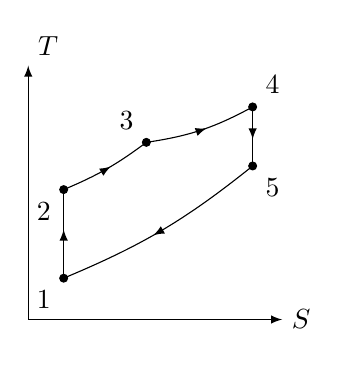
\begin{tikzpicture}[
	scale=\tabellenskalierung, every node/.style={scale=1},
  > = latex,
  dot/.style = {draw,fill,circle,inner sep=1pt},
  arrow inside/.style = {postaction=decorate,decoration={markings,mark=at position .55 with \arrow{>}}}
  ]
  	\draw[<->] (0,4.3) node[above right] {$T$} |- (4.3,0) node[right] {$S$};

	\coordinate (@1) at (0.6,0.7);
	\coordinate (@2) at (0.6,2.2);
	\coordinate (@3) at (2,3);
	\coordinate (@4) at (3.8,3.6);
	\coordinate (@5) at (3.8,2.6);

	\node[dot,label={below left:$1$}] at (@1) {};
	\node[dot,label={below left:$2$}] at (@2) {};
	\node[dot,label={above left:$3$}] at (@3) {};
	\node[dot,label={above right:$4$}] at (@4) {};
	\node[dot,label={below right:$5$}] at (@5) {};

  	\draw[arrow inside] (@1) to (@2);
	\draw[arrow inside] (@2) to[bend right=7] (@3);
	\draw[arrow inside] (@3) to[bend right=10] (@4);
  	\draw[arrow inside] (@4) to (@5);
	\draw[arrow inside] (@5) to[bend left=8] (@1);

\end{tikzpicture}
		&
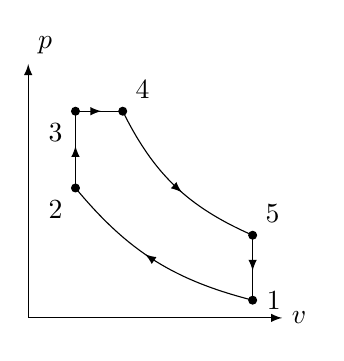
\begin{tikzpicture}[
	scale=\tabellenskalierung, every node/.style={scale=1},
  > = latex,
  dot/.style = {draw,fill,circle,inner sep=1pt},
  arrow inside/.style = {postaction=decorate,decoration={markings,mark=at position .55 with \arrow{>}}}
  ]
	\draw[<->] (0,4.3) node[above right] {$p$} |- (4.3,0) node[right] {$v$};

	\coordinate (@1) at (3.8,0.3);
	\coordinate (@2) at (0.8,2.2);
	\coordinate (@3) at (0.8,3.5);
	\coordinate (@4) at (1.6,3.5);
	\coordinate (@5) at (3.8,1.4);

	\node[dot,label={right:$1$}] at (@1) {};
	\node[dot,label={below left:$2$}] at (@2) {};
	\node[dot,label={below left:$3$}] at (@3) {};
	\node[dot,label={above right:$4$}] at (@4) {};
	\node[dot,label={above right:$5$}] at (@5) {};

	\draw[arrow inside] (@1) to[bend left=18] (@2);
  	\draw[arrow inside] (@2) to (@3);
  	\draw[arrow inside] (@3) to (@4);
	\draw[arrow inside] (@4) to[bend right=20] (@5);
  	\draw[arrow inside] (@5) to (@1);

\end{tikzpicture}
& 
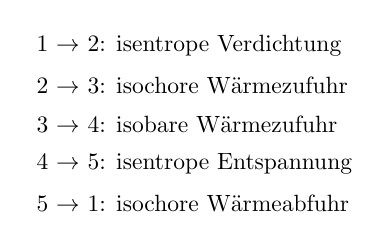
\begin{tikzpicture}
	[every node/.style={scale=0.85}]
	\draw (0,2) node[anchor=west] {1 $\rightarrow$ 2: isentrope Verdichtung};
	 \draw (0,1.5) node[anchor=west] {2 $\rightarrow$ 3: isochore Wärmezufuhr};
	 \draw (0,1) node[anchor=west] {3 $\rightarrow$ 4: isobare Wärmezufuhr}; 
	 \draw (0,0.5) node[anchor=west] {4 $\rightarrow$ 5: isentrope Entspannung}; 
	 \draw (0,0) node[anchor=west] {5 $\rightarrow$ 1: isochore Wärmeabfuhr};
\end{tikzpicture}
&
	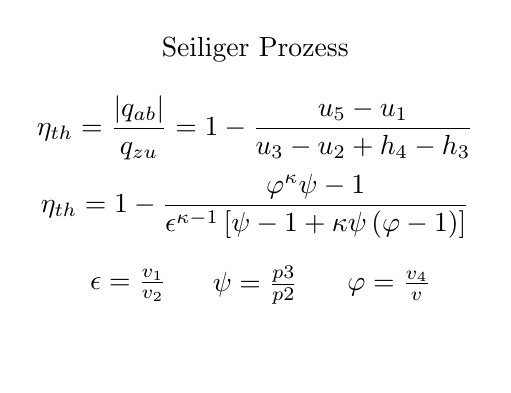
\begin{tikzpicture}
		\draw (1,4) node {Seiliger Prozess};
		\draw (1,3) node {$\displaystyle \eta_{th} =  \frac{|q_{ab}|}{q_{zu}} = 1 - \frac{u_5-u_1}{u_3 - u_2 + h_4 - h_3}$};
		\draw (1,2) node {$\displaystyle	\eta_{th} = 1 - \frac{\varphi^\kappa \psi - 1}{\epsilon^{\kappa-1}\left[\psi - 1 + \kappa \psi \left(\varphi -1 \right)\right]}$ };
		\draw (0,1) node[left] {$\epsilon = \frac{v_1}{v_2} $};
		\draw (1,1) node {$\psi     = \frac{p3}{p2}   $};
		\draw (2.7,1) node {$\varphi  = \frac{v_4}{v}   $};
		\draw (1,0);
	\end{tikzpicture}
\\ \hline
%\subsection{Otto-Prozess}

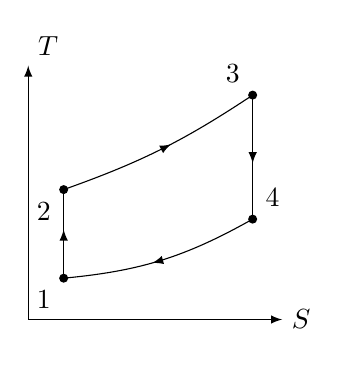
\begin{tikzpicture}[
	scale=\tabellenskalierung, every node/.style={scale=1},
  > = latex,
  dot/.style = {draw,fill,circle,inner sep=1pt},
  arrow inside/.style = {postaction=decorate,decoration={markings,mark=at position .55 with \arrow{>}}}
  ]
  	\draw[<->] (0,4.3) node[above right] {$T$} |- (4.3,0) node[right] {$S$};

	\coordinate (@1) at (0.6,0.7);
	\coordinate (@2) at (0.6,2.2);
	\coordinate (@3) at (3.8,3.8);
	\coordinate (@4) at (3.8,1.7);

	\node[dot,label={below left:$1$}] at (@1) {};
	\node[dot,label={below left:$2$}] at (@2) {};
	\node[dot,label={above left:$3$}] at (@3) {};
	\node[dot,label={above right:$4$}] at (@4) {};

  	\draw[arrow inside] (@1) to (@2);
	\draw[arrow inside] (@2) to[bend right=7] (@3);
	\draw[arrow inside] (@3) to (@4);
	\draw[arrow inside] (@4) to[bend left=12] (@1);

\end{tikzpicture}
&
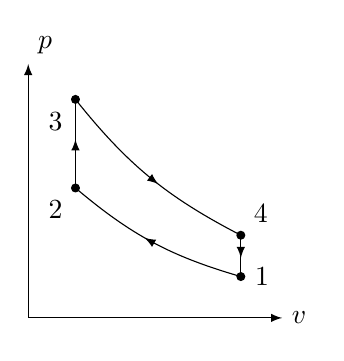
\begin{tikzpicture}[
	scale=\tabellenskalierung, every node/.style={scale=1},
  > = latex,
  dot/.style = {draw,fill,circle,inner sep=1pt},
  arrow inside/.style = {postaction=decorate,decoration={markings,mark=at position .55 with \arrow{>}}}
  ]
	\draw[<->] (0,4.3) node[above right] {$p$} |- (4.3,0) node[right] {$v$};

	\coordinate (@1) at (3.6,0.7);
	\coordinate (@2) at (0.8,2.2);
	\coordinate (@3) at (0.8,3.7);
	\coordinate (@4) at (3.6,1.4);

	\node[dot,label={right:$1$}] at (@1) {};
	\node[dot,label={below left:$2$}] at (@2) {};
	\node[dot,label={below left:$3$}] at (@3) {};
	\node[dot,label={above right:$4$}] at (@4) {};

	\draw[arrow inside] (@1) to[bend left=12] (@2);
  	\draw[arrow inside] (@2) to (@3);
	\draw[arrow inside] (@3) to[bend right=12] (@4);
	\draw[arrow inside] (@4) to (@1);

\end{tikzpicture}
& 
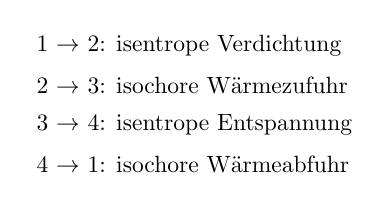
\begin{tikzpicture}
	[every node/.style={scale=0.85}]
	\draw (0,2) node[anchor=west] {1 $\rightarrow$ 2: isentrope Verdichtung};
	 \draw (0,1.5) node[anchor=west] {2 $\rightarrow$ 3: isochore Wärmezufuhr};
	 \draw (0,1) node[anchor=west] {3 $\rightarrow$ 4: isentrope Entspannung};
	 \draw (0,0.5) node[anchor=west] {4 $\rightarrow$ 1: isochore Wärmeabfuhr};
\end{tikzpicture}
&
	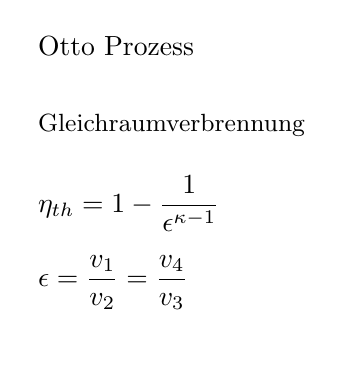
\begin{tikzpicture}
		\draw (1,4) node[anchor=west] {Otto Prozess};
		\draw (1,3) node[anchor=west] {\small Gleichraumverbrennung};
		\draw (1,2) node[anchor=west] {$\displaystyle \eta_{th} = 1 -\frac{1}{\epsilon^{\kappa  -1}} $};
		\draw (1,1) node[anchor=west] { $\displaystyle \epsilon	= \frac{v_1}{v_2} = \frac{v_4}{v_3} $ };
		\draw (1,0);
	\end{tikzpicture}

\\ \hline

%\subsection{Diesel-Prozess}

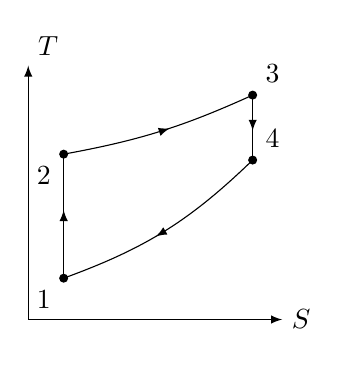
\begin{tikzpicture}[
	scale=\tabellenskalierung, every node/.style={scale=1},
  > = latex,
  dot/.style = {draw,fill,circle,inner sep=1pt},
  arrow inside/.style = {postaction=decorate,decoration={markings,mark=at position .55 with \arrow{>}}}
  ]
  	\draw[<->] (0,4.3) node[above right] {$T$} |- (4.3,0) node[right] {$S$};

	\coordinate (@1) at (0.6,0.7);
	\coordinate (@2) at (0.6,2.8);
	\coordinate (@3) at (3.8,3.8);
	\coordinate (@4) at (3.8,2.7);

	\node[dot,label={below left:$1$}] at (@1) {};
	\node[dot,label={below left:$2$}] at (@2) {};
	\node[dot,label={above right:$3$}] at (@3) {};
	\node[dot,label={above right:$4$}] at (@4) {};

  	\draw[arrow inside] (@1) to (@2);
	\draw[arrow inside] (@2) to[bend right=7] (@3);
	\draw[arrow inside] (@3) to (@4);
	\draw[arrow inside] (@4) to[bend left=12] (@1);

\end{tikzpicture}
&
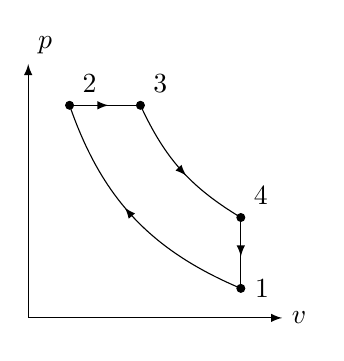
\begin{tikzpicture}[
	scale=\tabellenskalierung, every node/.style={scale=1},
  > = latex,
  dot/.style = {draw,fill,circle,inner sep=1pt},
  arrow inside/.style = {postaction=decorate,decoration={markings,mark=at position .55 with \arrow{>}}}
  ]
	\draw[<->] (0,4.3) node[above right] {$p$} |- (4.3,0) node[right] {$v$};

	\coordinate (@1) at (3.6,0.5);
	\coordinate (@2) at (0.7,3.6);
	\coordinate (@3) at (1.9,3.6);
	\coordinate (@4) at (3.6,1.7);

	\node[dot,label={right:	     $1$}] at (@1) {};
	\node[dot,label={above right:$2$}] at (@2) {};
	\node[dot,label={above right:$3$}] at (@3) {};
	\node[dot,label={above right:$4$}] at (@4) {};

	\draw[arrow inside] (@1) to[bend left=24] 	(@2);
  	\draw[arrow inside] (@2) to 			(@3);
	\draw[arrow inside] (@3) to[bend right=17] 	(@4);
	\draw[arrow inside] (@4) to 			(@1);

\end{tikzpicture}
& 
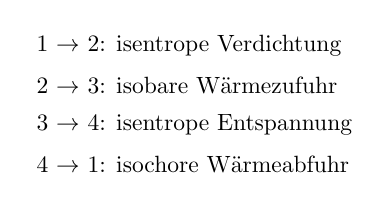
\begin{tikzpicture}
	[every node/.style={scale=0.85}]
	\draw (0,2) node[anchor=west] {1 $\rightarrow$ 2: isentrope Verdichtung};
	 \draw (0,1.5) node[anchor=west] {2 $\rightarrow$ 3: isobare Wärmezufuhr};
	 \draw (0,1) node[anchor=west] {3 $\rightarrow$ 4: isentrope Entspannung}; 
	 \draw (0,0.5) node[anchor=west] {4 $\rightarrow$ 1: isochore Wärmeabfuhr}; 
\end{tikzpicture}
&

	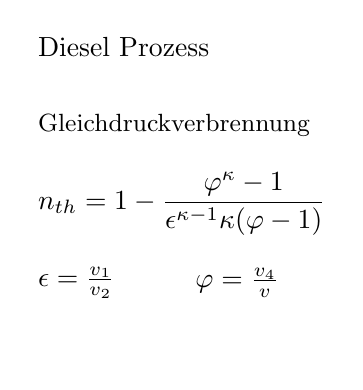
\begin{tikzpicture}
		\draw (1,4) node[anchor=west] {Diesel Prozess};
		\draw (1,3) node[anchor=west] {\small Gleichdruckverbrennung};
		\draw (1,2) node[anchor=west] {$\displaystyle	n_{th} = 1 - \frac{\varphi^\kappa - 1}{\epsilon^{\kappa -1}\kappa(\varphi - 1)}$};
		\draw (1,1) node[left,anchor=west] {$\epsilon = \frac{v_1}{v_2} $};
		\draw (3,1) node[right,anchor=west] {$\varphi  = \frac{v_4}{v}   $};
		\draw (1,0);
	\end{tikzpicture}
\\ \hline
%\subsection{Stirling-Prozess}

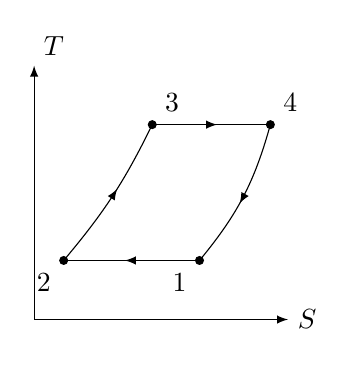
\begin{tikzpicture}[
	scale=\tabellenskalierung, every node/.style={scale=1},
  > = latex,
  dot/.style = {draw,fill,circle,inner sep=1pt},
  arrow inside/.style = {postaction=decorate,decoration={markings,mark=at position .55 with \arrow{>}}}
  ]
  	\draw[<->] (0,4.3) node[above right] {$T$} |- (4.3,0) node[right] {$S$};

	\coordinate (@1) at (2.8,1);
	\coordinate (@2) at (0.5,1);
	\coordinate (@3) at (2.0,3.3);
	\coordinate (@4) at (4,3.3);

	\node[dot,label={below  left:$1$}] at (@1) {};
	\node[dot,label={below  left:$2$}] at (@2) {};
	\node[dot,label={above right:$3$}] at (@3) {};
	\node[dot,label={above right:$4$}] at (@4) {};

  	\draw[arrow inside] (@1) to (@2);
	\draw[arrow inside] (@2) to[bend right=7] (@3);
	\draw[arrow inside] (@3) to (@4);
	\draw[arrow inside] (@4) to[bend left=12] (@1);

\end{tikzpicture}
&
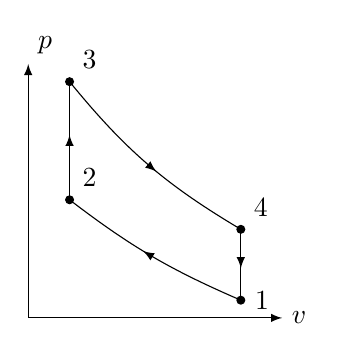
\begin{tikzpicture}[
	scale=\tabellenskalierung, every node/.style={scale=1},
  > = latex,
  dot/.style = {draw,fill,circle,inner sep=1pt},
  arrow inside/.style = {postaction=decorate,decoration={markings,mark=at position .55 with \arrow{>}}}
  ]
	\draw[<->] (0,4.3) node[above right] {$p$} |- (4.3,0) node[right] {$v$};

	\coordinate (@1) at (3.6,0.3);
	\coordinate (@2) at (0.7,2.0);
	\coordinate (@3) at (0.7,4);
	\coordinate (@4) at (3.6,1.5);

	\node[dot,label={right:$1$}] at (@1) {};
	\node[dot,label={above right:$2$}] at (@2) {};
	\node[dot,label={above right:$3$}] at (@3) {};
	\node[dot,label={above right:$4$}] at (@4) {};

	\draw[arrow inside] (@1) to[bend left=7] (@2);
  	\draw[arrow inside] (@2) to (@3);
	\draw[arrow inside] (@3) to[bend right=10] (@4);
	\draw[arrow inside] (@4) to (@1);

\end{tikzpicture}
& 
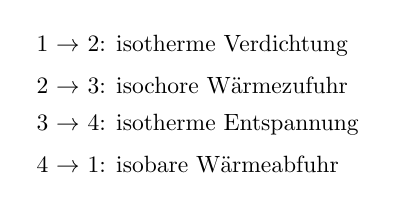
\begin{tikzpicture}
	[every node/.style={scale=0.85}]
	\draw (0,2) node[anchor=west] {1 $\rightarrow$ 2: isotherme Verdichtung};
	 \draw (0,1.5) node[anchor=west] {2 $\rightarrow$ 3: isochore Wärmezufuhr};
	 \draw (0,1) node[anchor=west] {3 $\rightarrow$ 4: isotherme Entspannung}; 
	 \draw (0,0.5) node[anchor=west] {4 $\rightarrow$ 1: isobare Wärmeabfuhr}; 
\end{tikzpicture}
&

	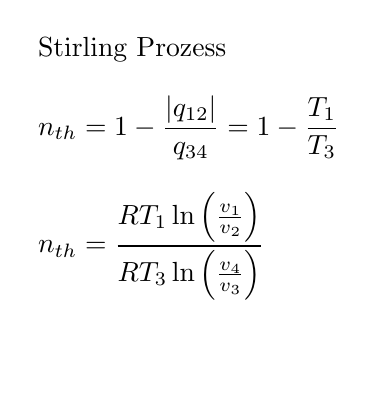
\begin{tikzpicture}
		\draw (1,4) node[anchor=west] {Stirling Prozess};
		\draw (1,3) node[anchor=west] {$\displaystyle	n_{th} = 1 - \frac{|q_{12}|}{q_{34}} = 1 - \frac{T_1}{T_3}$};
		\draw (1,1.5) node[anchor=west] {$\displaystyle	n_{th}  = \frac{RT_1 \ln\left(\frac{v_1}{v_2}\right)}{RT_3 \ln \left(\frac{v_4}{v_3}\right)}$};
		\draw (1,0);
\end{tikzpicture}  
\\ \hline
%\subsection{Joule-Prozess}


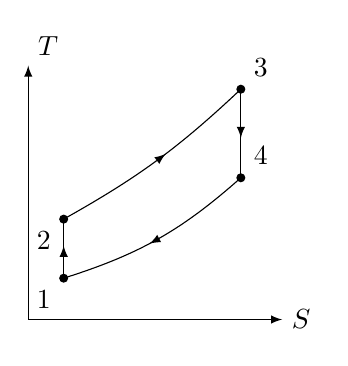
\begin{tikzpicture}[
	scale=\tabellenskalierung, every node/.style={scale=1},
  > = latex,
  dot/.style = {draw,fill,circle,inner sep=1pt},
  arrow inside/.style = {postaction=decorate,decoration={markings,mark=at position .55 with \arrow{>}}}
  ]
  	\draw[<->] (0,4.3) node[above right] {$T$} |- (4.3,0) node[right] {$S$};

	\coordinate (@1) at (0.6,0.7);
	\coordinate (@2) at (0.6,1.7);
	\coordinate (@3) at (3.6,3.9);
	\coordinate (@4) at (3.6,2.4);

	\node[dot,label={below left:$1$}] at (@1) {};
	\node[dot,label={below left:$2$}] at (@2) {};
	\node[dot,label={above right:$3$}] at (@3) {};
	\node[dot,label={above right:$4$}] at (@4) {};

  	\draw[arrow inside] (@1) to (@2);
	\draw[arrow inside] (@2) to[bend right=7] (@3);
	\draw[arrow inside] (@3) to (@4);
	\draw[arrow inside] (@4) to[bend left=12] (@1);

\end{tikzpicture}
&
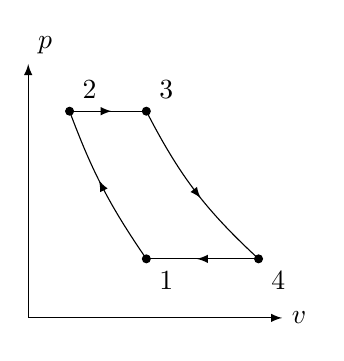
\begin{tikzpicture}[
	scale=\tabellenskalierung, every node/.style={scale=1},
  > = latex,
  dot/.style = {draw,fill,circle,inner sep=1pt},
  arrow inside/.style = {postaction=decorate,decoration={markings,mark=at position .55 with \arrow{>}}}
  ]
	\draw[<->] (0,4.3) node[above right] {$p$} |- (4.3,0) node[right] {$v$};

	\coordinate (@1) at (2,1);
	\coordinate (@2) at (0.7,3.5);
	\coordinate (@3) at (2,3.5);
	\coordinate (@4) at (3.9,1);

	\node[dot,label={below right:$1$}] at (@1) {};
	\node[dot,label={above right:$2$}] at (@2) {};
	\node[dot,label={above right:$3$}] at (@3) {};
	\node[dot,label={below right:$4$}] at (@4) {};

	\draw[arrow inside] (@1) to[bend left=7] (@2);
  	\draw[arrow inside] (@2) to (@3);
	\draw[arrow inside] (@3) to[bend right=10] (@4);
	\draw[arrow inside] (@4) to (@1);

\end{tikzpicture}
& 
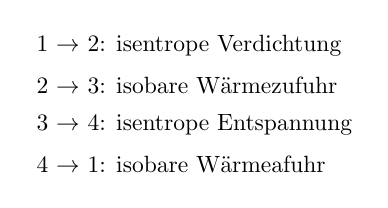
\begin{tikzpicture}
	[every node/.style={scale=0.85}]
	\draw (0,2) node[anchor=west] {1 $\rightarrow$ 2: isentrope Verdichtung};
	 \draw (0,1.5) node[anchor=west] {2 $\rightarrow$ 3: isobare Wärmezufuhr};
	 \draw (0,1) node[anchor=west] {3 $\rightarrow$ 4: isentrope Entspannung}; 
	 \draw (0,0.5) node[anchor=west] {4 $\rightarrow$ 1: isobare Wärmeafuhr}; 
\end{tikzpicture}
&

	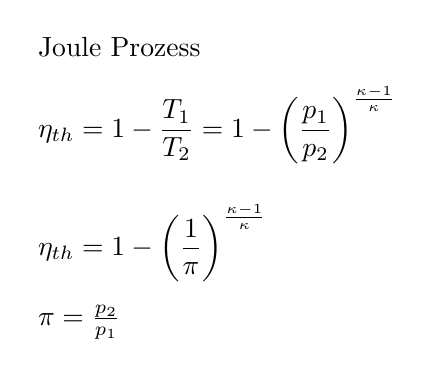
\begin{tikzpicture}
		\draw (1,4) node[anchor=west] {Joule Prozess};
		\draw (1,3) node[anchor=west] {$\displaystyle \eta_{th} = 1 - \frac{T_1}{T_2} = 1 - \left(\frac{p_1}{p_2}\right)^{\frac{\kappa-1}{\kappa}}$};
		\draw (1,1.5) node[anchor=west] {$\displaystyle \eta_{th}  = 1 - \left( \frac{1}{\pi}\right)^{\frac{\kappa -1 }{\kappa}}$};
		\draw (1,0.5) node[anchor=west] {$\pi = \frac{p_2}{p_1}$};
		\draw (1,0);
	\end{tikzpicture}
\\ \hline
%\subsection{Ericsson-Prozess}

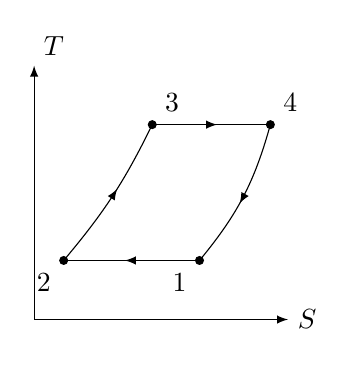
\begin{tikzpicture}[
	scale=\tabellenskalierung, every node/.style={scale=1},
  > = latex,
  dot/.style = {draw,fill,circle,inner sep=1pt},
  arrow inside/.style = {postaction=decorate,decoration={markings,mark=at position .55 with \arrow{>}}}
  ]
  	\draw[<->] (0,4.3) node[above right] {$T$} |- (4.3,0) node[right] {$S$};

	\coordinate (@1) at (2.8,1);
	\coordinate (@2) at (0.5,1);
	\coordinate (@3) at (2.0,3.3);
	\coordinate (@4) at (4,3.3);

	\node[dot,label={below left:$1$}] at (@1) {};
	\node[dot,label={below left:$2$}] at (@2) {};
	\node[dot,label={above right:$3$}] at (@3) {};
	\node[dot,label={above right:$4$}] at (@4) {};

  	\draw[arrow inside] (@1) to (@2);
	\draw[arrow inside] (@2) to[bend right=7] (@3);
	\draw[arrow inside] (@3) to (@4);
	\draw[arrow inside] (@4) to[bend left=12] (@1);

\end{tikzpicture}
&
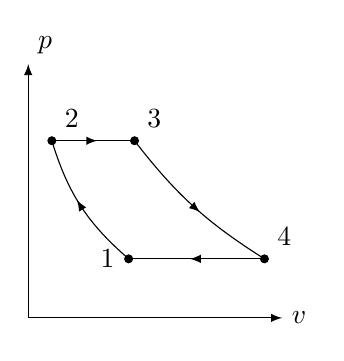
\begin{tikzpicture}[
	scale=\tabellenskalierung, every node/.style={scale=1},
  > = latex,
  dot/.style = {draw,fill,circle,inner sep=1pt},
  arrow inside/.style = {postaction=decorate,decoration={markings,mark=at position .55 with \arrow{>}}}
  ]
	\draw[<->] (0,4.3) node[above right] {$p$} |- (4.3,0) node[right] {$v$};

	\coordinate (@1) at (1.7,1);
	\coordinate (@2) at (0.4,3.0);
	\coordinate (@3) at (1.8,3);
	\coordinate (@4) at (4,1);

	\node[dot,label={left:$1$}] at (@1) {};
	\node[dot,label={above right:$2$}] at (@2) {};
	\node[dot,label={above right:$3$}] at (@3) {};
	\node[dot,label={above right:$4$}] at (@4) {};

	\draw[arrow inside] (@1) to[bend left=16] (@2);
  	\draw[arrow inside] (@2) to (@3);
	\draw[arrow inside] (@3) to[bend right=10] (@4);
	\draw[arrow inside] (@4) to (@1);

\end{tikzpicture}
& 
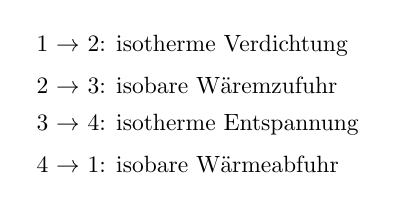
\begin{tikzpicture}
	[every node/.style={scale=0.85}]
	\draw (0,2) node[anchor=west] {1 $\rightarrow$ 2: isotherme Verdichtung};
	 \draw (0,1.5) node[anchor=west] {2 $\rightarrow$ 3: isobare Wäremzufuhr};
	 \draw (0,1) node[anchor=west] {3 $\rightarrow$ 4: isotherme Entspannung}; 
	 \draw (0,0.5) node[anchor=west] {4 $\rightarrow$ 1: isobare Wärmeabfuhr}; 
\end{tikzpicture}
&

	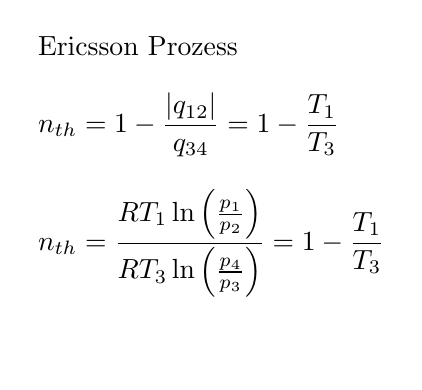
\begin{tikzpicture}
		\draw (1,4) node[anchor=west] {Ericsson Prozess};
		\draw (1,3) node[anchor=west] {$\displaystyle	n_{th} = 1 - \frac{|q_{12}|}{q_{34}} = 1 - \frac{T_1}{T_3}$};
		\draw (1,1.5) node[anchor=west] {$\displaystyle	n_{th} = \frac{RT_1 \ln\left(\frac{p_1}{p_2}\right)}{RT_3 \ln \left(\frac{p_4}{p_3}\right)}= 1 - \frac{T_1}{T_3}$};
		\draw (1,0);
\end{tikzpicture}  
\end{tabular}
\end{table}

\onecolumn

%       ____    __           __             ______              
%      /  _/___/ /__  ____ _/ /__  _____   / ____/___ ______    
%      / // __  / _ \/ __ `/ / _ \/ ___/  / / __/ __ `/ ___/    
%    _/ // /_/ /  __/ /_/ / /  __(__  )  / /_/ / /_/ (__  )     
%   /___/\__,_/\___/\__,_/_/\___/____/   \____/\__,_/____/      
                                                               
\begin{landscape}
	\LARGE
	Ideales Gas 
	\\\\
	\renewcommand{\arraystretch}{2}
\begin{tabular}{l|l|l|l|l|l}
& Isothermo
& Isobare  
& Isochore  
& Isentrop  
& Polytrope 
\\ \hline
  konstant:  
& T ($n = 1$) 
& p ($n = 0$) 
& v ($n \rightarrow \infty$) 
& $\delta q=0$ ($n = \kappa$) 
& $pv^n$  
\\ \hline
	
& -  
& -  
& -  
& $p_1 v_1^{\kappa} = p_2 v_2^{\kappa}$  
& $v_1^{n} = p_2 v_2^{n}$  
\\ \hline

& $p_1 v_1 = p_2 v_2$  
& $\frac{v_1}{v_2} = \frac{T_1}{T_2}$  
& $\frac{p_1}{T_1} = \frac{p_2}{T_2}$  
& $T_1 v_1^{\kappa - 1} = T_2 v_2^{\kappa -1}$   
& $T_1 v_1^{n - 1} = T_2 v_2^{n -1}$  
\\ \hline
	
& -  
& -  
& -  
%& $\small\xrightswishingghost{}$  
& $\frac{T_1^{\frac{\kappa}{\kappa -1}}}{p_1} = \frac{T_2^{\frac{\kappa}{\kappa -1}}}{p_2}$  
& $\frac{T_1^{\frac{n}{n -1}}}{p_1} = \frac{T_2^{\frac{n}{n -1}}}{p_2}$  
\\ \hline

	$p,v$

& $p = \frac{p_1 v_1}{v}$  
& $p = p_1$  
& $v = v_1$  
& $p = \frac{p_1 v_1^{\kappa}}{v^{\kappa}}$  
& $p = \frac{p_1 v_1^{n}}{v^{n}}$ 
\\ \hline

	$p,T$

& $p = \frac{p_1 v_1}{v}$  
& $p = p_1$  
& $p = \frac{p_1}{T_1}T$  
& $p = p_1  \left(\frac{T}{T_1}\right)^{\frac{\kappa}{\kappa -1}}$  
& $p = p_1 \left(\frac{T}{T_1}\right)^{\frac{n}{n -1}}$
\\ \hline

	$v,T$  

& $T = T_1$  
& $v = \frac{v_1}{T_1}T$  
& $v = v_1 $ 
& $T = T_1\left(\frac{v_1}{v}\right)^{\kappa - 1}$  
& $T = T_1 \left(\frac{v_1}{v}\right)^{n-1}$
\\ \hline

	$q_{12}$	

& $= p_1v_1 \ln \frac{p_1}{p_2}$  
& $= c_p(T_2 - T_1)$   
& $= c_v(T_2 - T_1)$  
& $= 0$   
&  $= c_v \frac{n-\kappa}{n-1}(T_2-T_1)$ 
\\ \hline

	$w_{V,12}$  

& $= -q_{12}$ 
& $= -p_1(v_2 - v_1)$  
& $= 0$  
& $= \frac{p_1 v_1}{k - 1}\left[\left(\frac{v_1}{v_2}\right)^{\kappa - 1} - 1\right]$  
& $= \frac{p_1 v_1}{n - 1}\left[\left(\frac{v_1}{v_2}\right)^{n-1} - 1\right]$ 
\\ \hline

	$s_2 - s_1$ 

& $= R \ln \left(\frac{p_1}{p_2}\right)$  
& $= c_p \ln \left(\frac{T_2}{T_1}\right)$  
& $= c_v \ln \left(\frac{T_2}{T_1}\right)$  
& $= 0$  
& $= c_v \frac{n - \kappa }{n - 1} \ln \left(\frac{T_2}{T_1}\right)$  
\\ 
\end{tabular}
\bigskip
\\\\
% _    __                  ____                _       __            __         
%| |  / /___ _____        / __ \___  _____    | |     / /___ _____ _/ /____     
%| | / / __ `/ __ \______/ / / / _ \/ ___/____| | /| / / __ `/ __ `/ / ___/_____
%| |/ / /_/ / / / /_____/ /_/ /  __/ /  /_____/ |/ |/ / /_/ / /_/ / (__  )_____/
%|___/\__,_/_/ /_/     /_____/\___/_/         |__/|__/\__,_/\__,_/_/____/       
%                                                                               
%   ______                
%  / ____/___ ______      
% / / __/ __ `/ ___/      
%/ /_/ / /_/ (__  )       
%\____/\__,_/____/        

\Large
Van-Der-Waals-Gas  
\\

	\begin{tabular}{l|l|l|l|l}
		
& Isotherme 
& Isobare 
& Isochore 
& Isentrop 
\\ \hline
		konstant: 
& T 
& p 
& v  
& $\delta = 0$ 
\\ \hline
		
& \thead{\Large$(p_1 + \frac{a}{v^2})(v_1-b)$ \\\Large $= (p_2 + \frac{a}{v^2})(v_2-b)$}
& \Large$\frac{RT_1}{v_1-b} - \frac{a}{v_1^2} = \frac{RT_2}{v-b} - \frac{a}{v_2^2}$ 
& $\frac{p_1 + \frac{a}{v_1^2}}{T_1} = \frac{p_2 + \frac{a}{v_1^2}}{T_2}$  
& \thead{\large $(p_1 + \frac{a}{v^2}) (v_1-b)^{\frac{c_v + R}{c_v}}$ \\\large $ = (p + \frac{a}{v^2}) (v_2-b)^{\frac{c_v + R}{c_v}},$ \\ \large $ \quad T_1(v_1-b)^{R/c_v} = T_2 (v_2-b)^{R/c_v}$}  
\\ \hline

		$p,v$ 

& $p = (p + \frac{a}{v^2}) \frac{v_u}{v-b} - \frac{a}{v^2}$ 
& $p = p_1$  
& $v = v_1$ 
& $p = - \frac{a}{v^2} + (p_1 + \frac{a}{v^2}) \left(\frac{v_1-b}{v_m}\right)^{\frac{v_v + R }{R}}$ 
\\ \hline

		$p,T$ 

& $T = T_1$ 
& $p = p_1$ 
& $p = \frac{T}{T_1} (p_1 + \frac{a}{v^2}) - \frac{a}{v_1^2}$ 
& $p = - \frac{a}{v^2}+ (p_1 + \frac{a}{v^2}) \left(\frac{T}{T_1}\right)^\frac{c_v+R}{R}$ 
\\ \hline

		$v,T$ 

& $T = T_1$ 
& $T = T_1 \frac{v-b}{v_1-b} + \frac{a}{R}(v-b) \left(\frac{1}{v^2} - \frac{1}{v_1^2}\right)$ 
& $v = v_1$  
& $T = T_1 \left(\frac{v_1-b}{v-b}\right)^\frac{R}{c_v}$ 
\\ \hline

		$q_{12}$ 

& $= RT_1 \ln \left(\frac{v_2-b}{v_1-b}\right)$ 
& $= \frac{a}{v_1} - \frac{a}{v_2} + c_v(T_2 - T_1) + p_1(v_2 - v_1)$ 
& $= c_v(T_2 - T_1)$  
& $= 0$  
\\ \hline

		$w_{V,12}$ 

& $= -RT_1 \ln \left(\frac{v_2-b}{v_1-b}\right) + \frac{a}{v_1} - \frac{a}{v_2}$ 
& $= -p_1(v_2-v_1)$ 
& $= 0$  
& $= \frac{a}{v_1} - \frac{a}{v_2} + c_v(T_2 - T_1)$ 
\\ \hline

		$s_2 - s_1$ 

& $= R\ln \left(\frac{v_2-b}{v_1-b}\right)$ 
& $= c_v \ln \left(\frac{T_2}{T_1}\right) + R \ln \left(\frac{v_2-b}{v_1-b}\right)$ 
& $= c_v \ln \left(\frac{T_2}{T_1}\right)$ 
& $= 0$ 
\\
\end{tabular}
\end{landscape}

%   _____ __        ________                   __     
%  / ___// /_____  / __/ __/      _____  _____/ /____ 
%  \__ \/ __/ __ \/ /_/ /_| | /| / / _ \/ ___/ __/ _ \
% ___/ / /_/ /_/ / __/ __/| |/ |/ /  __/ /  / /_/  __/
%/____/\__/\____/_/ /_/   |__/|__/\___/_/   \__/\___/ 
%	                                                     
%    _______       _                    ______              
%   / ____(_)___  (_)___ ____  _____   / ____/___ _________ 
%  / __/ / / __ \/ / __ `/ _ \/ ___/  / / __/ __ `/ ___/ _ \
% / /___/ / / / / / /_/ /  __/ /     / /_/ / /_/ (__  )  __/
%/_____/_/_/ /_/_/\__, /\___/_/      \____/\__,_/____/\___/ 
%                /____/                                     
%
\section{Stoffwerte einiger Gase}

\begin{center}

\begin{tabular}{l|l|r|r|r|r|r|r}
  Bezeichnung	&	Symbol	&Molmasse 	&Gaskonstante	&	Dichte 	& $c_p$ & $c_v$ &$\kappa$ \\
		&		&[kg/kmol]	&[J/(kg K)]	& 	[kg/$m^3$]	& [J/(kg K)]	& [J/(kg,K)] & \\
	&&&&&&\\
Acetylen	&$	C_2H_2	$&	26.038	&	319.3	&	1.16 	&	1616	&	1278	&	1.26 \\
Ammoniak	&$	NH_3	$&	17.031	&	488.2	&	0.76 	&	2056	&	1526	&	1.35 \\
Argon		&$	Ar	$&	39.948	&	208.1	&	1.76 	&	519	&	309	&	1.68 \\
Äthan		&$	C_2H_6	$&	30.070	&	276.5	&	1.34 	&	1650	&	1355	&	1.22 \\
Butan		&$	C_4H_10	$&	58.124	&	143.0	&	2.67 	&	1599	&	1410	&	1.13 \\
Chlor		&$	C_l2	$&	56.108	&	117.3	&	3.17 	&	473	&	343	&	1.38 \\
Chlorwasserstoff&$	HCl	$&	70.906	&	228.0	&	1.62 	&	795	&	556	&	1.43 \\
Helium		&$	He	$&	4.003	&	2077.0	&	0.18 	&	5200	&	3124	&	1.66 \\
Kohlendioxid	&$	CO_2	$&	44.010	&	188.9	&	1.95 	&	816	&	618	&	1.32 \\
Kohlenmonoxid	&$	CO	$&	28.010	&	296.8	&	1.23 	&	1038	&	739	&	1.40 \\
Luft		&--		&	28.964	&	287.1	&	1.28 	&	1006	&	718	&	1.40 \\
Methan		&$	CH_4	$&	16.043	&	518.3	&	0.71 	&	2165	&	1638	&	1.32 \\
Propan		&$	C_3H_8	$&	44.097	&	188.5	&	1.99 	&	1549	&	1331	&	1.16 \\
Sauerstoff	&$	O_2	$&	31.999	&	259.8	&	1.41 	&	909	&	647	&	1.40 \\
Stickstoff	&$	N_2	$&	28.013	&	296.8	&	1.23 	&	1038	&	739	&	1.40 \\
Wasserstoff	&$	H_2	$&	2.016	&	4124.2	&	0.09 	&	14050	&	9926	&	1.42 \\
Xenon		&$	Xe	$&	131.300	&	63.3	&	5.82 	&	159	&	93	&	1.71 \\
	Ideales Gas	&		 &		&	8.3143[J/mol K]	&		&		& \\\\
  \multicolumn{8}{c}{Dichte, $c_p$ und $c_v$ bei: $T = 273,15 K,\; p =
  1\operatorname{bar}$}
\end{tabular}

\end{center}
%   _____ __        ________    __      __                     _       _                
%  / ___// /_____  / __/ __/___/ /___ _/ /____  ____     ___  (_)___  (_)___ ____  _____
%  \__ \/ __/ __ \/ /_/ /_/ __  / __ `/ __/ _ \/ __ \   / _ \/ / __ \/ / __ `/ _ \/ ___/
% ___/ / /_/ /_/ / __/ __/ /_/ / /_/ / /_/  __/ / / /  /  __/ / / / / / /_/ /  __/ /    
%/____/\__/\____/_/ /_/  \__,_/\__,_/\__/\___/_/ /_/   \___/_/_/ /_/_/\__, /\___/_/     
%                                                                    /____/             
%   _____ __        ________   
%  / ___// /_____  / __/ __/__ 
%  \__ \/ __/ __ \/ /_/ /_/ _ \
% ___/ / /_/ /_/ / __/ __/  __/
%/____/\__/\____/_/ /_/  \___/ 
%										                                  
%
\section{Stoffdaten einiger Stoffe}

\begin{center}

\begin{tabular}{l|r|r|r|r|r}
	Name	& chemische &	 Molmasse  	& Normal-& kritische & kritischer \\
Name	& Formel&	 [kg/kmol]	& Siedepunkt [\textcelsius]	& Temperatur [\textcelsius]	& Druck [MPa] 	\\
		&			&			&			&		&	 	\\
Wasserstoff	&	$H_2$		&		2.02	&		-252.9	&	-240.0	&	1.32 	\\
Helium		&	$He$		&		4.00	&		-268.9	&	-268.0	&	0.23 	\\
Ammoniak	&	$NH_3$		&		17.03	&		-33.3	&	132.3	&	11.33 	\\
Wasser		&	$H_2O$		&		18.02	&		100.0	&	373.9	&	22.06 	\\
Luft		&\begin{tabular}{r} $78\%$ 	\\ $N_2 21\%$ \\ $O_2. 1\% Ar.+$\end{tabular}&	28.96	&	-194.2	&-140.4	&3.84 \\
Kohlendioxid	&	$CO_2$		&		44.01	&		-78.4	&	31.0	&	7.38 	\\
Methan		&	$CH_4$		&		16.04	&		-161.5	&	-82.6	&	4.60 	\\
Äthan		&	$C_2H_6$	&		30.07	&		-88.6	&	32.2	&	4.87 	\\
Propan		&	$C_3H_8$	&		44.10	&		-42.1	&	96.7	&	4.25 	\\
R134a		&	$CH_2FCF_3$	&		102.03	&		-26.1	&	101.1	&	4.06 	\\
\end{tabular} \\
\end{center}


% _____         __    __                             __     
%/__  /  ____ _/ /_  / /__  ____ _      _____  _____/ /____ 
%  / /  / __ `/ __ \/ / _ \/ __ \ | /| / / _ \/ ___/ __/ _ \
% / /__/ /_/ / / / / /  __/ / / / |/ |/ /  __/ /  / /_/  __/
%/____/\__,_/_/ /_/_/\___/_/ /_/|__/|__/\___/_/   \__/\___/ 
%                                                           
%    ____                __    __          __          ______ 
%   / __/__  __  _______/ /_  / /____     / /   __  __/ __/ /_
%  / /_/ _ \/ / / / ___/ __ \/ __/ _ \   / /   / / / / /_/ __/
% / __/  __/ /_/ / /__/ / / / /_/  __/  / /___/ /_/ / __/ /_  
%/_/  \___/\__,_/\___/_/ /_/\__/\___/  /_____/\__,_/_/  \__/  
%
                                                             
\section{Zahlenwerte feuchte Luft}

\begin{center}
\begin{tabular}{l|r|r|r|r}
Bezeichnung& Formelzeichen& Zahlenwert& Dimension \\
	&&&& \\
Molmasse der Luft& ML& 28,96& kg/ kmol \\
Molmasse des Wassers& MH2O& 18,02& kg/ kmol \\
spezifische Gaskonstante der Luft& RL& 0,287& kJ/ (kg K) \\
spezifische Gaskonstante des Dampfes& RD& 0,461& kJ/ (kg K) \\
spezifische Wärmekapazität der Luft& cpL& 1,006& kJ/ (kg K) \\
spezifische Wärmekapazität des Dampfes& cpD& 1,92& kJ/ (kg K) \\
spezifische Wärmekapazität des Wassers& cW& 4,182& kJ/ (kg K) \\
spezifische Wärmekapazität des Eises& cE& 2,1& kJ/ (kg K) \\
Verdampfungsenthalpie des Wassers bei 0 °C& rD& 2500& kJ/ kg \\
Schmelzenthalpie des Eises bei 0 °C& rE& 334& kJ/ kg \\
\end{tabular}


\end{center}

%   ____  __         __                 
%  / __ \/ /_  _____/ /____  __________ 
% / / / / __ \/ ___/ //_/ / / / ___/ _ \
%/ /_/ / /_/ (__  ) ,< / /_/ / /  /  __/
%\____/_.___/____/_/|_|\__,_/_/   \___/ 
%                                             
% _____                                                   __     /\// /|___/|              
%/__  /  __  ___________ _____ ___  ____ ___  ___  ____  / /_  _//\/ | __  /___  ____ ____ 
%  / /  / / / / ___/ __ `/ __ `__ \/ __ `__ \/ _ \/ __ \/ __ \/ _ | / /_/ / __ \/ __ `/ _ \
% / /__/ /_/ (__  ) /_/ / / / / / / / / / / /  __/ / / / / / / __ |/___  / / / / /_/ /  __/
%/____/\__,_/____/\__,_/_/ /_/ /_/_/ /_/ /_/\___/_/ /_/_/ /_/_/ |_|/   |/_/ /_/\__, /\___/ 
%                                                                             /____/       
%
\section{Obskure Zusammenhänge}


Aus Anhang B
\begin{align}
	dV	&= \left(\frac{\partial V}{\partial T}\right)_{p} dT 
	+ \left(\frac{\partial V}{\partial p}\right)_{T,n}  
	+ \sum_{k=1}^{K} \left(\frac{\partial V}{\partial n_k}\right)_{T,p} dkn_k \\
	dS	&= \left(\frac{nC_{p,m}}{T} \right) dT 
	- \left(\frac{\partial V}{\partial T}\right)_{p,n} dp 
	+ \sum_{k=1}^{K} \left(\frac{\partial \mu_k}{\partial T}\right)_{p,n} dn_k \\
	dU	&= \left[nC_{p,m} 
	- p \left(\frac{\partial V}{\partial T}\right)_{p,n}\right]dT 
	-  \left[p\left(\frac{\partial V}{\partial p}\right)_{T,n} 
	+ T \left(\frac{\partial V}{\partial T}\right)_{p,n} \right]dp 
	+ \sum_{k=1}^{K} \left[ \mu_k 
	-T \left(\frac{\partial \mu_k}{\partial T}\right)_{p,n} 
	- p \left(\frac{\partial V}{\partial n_k}\right)_{T,p,n} \right]dn_k \\
	dH 	&= nC_{p,m} dT 
	+ \left[V T \left(\frac{\partial V}{\partial T}\right)_{p,n}\right] 
	+ \sum_{k=1}^{K} \left[ \mu_k 
	- T \left(\frac{\partial \mu_k}{\partial T}\right)_{p,n} \right] dn_k  \\
	dF	&= 
	-\left[S 
	+ p \left(\frac{\partial V}{\partial T}\right)_{p,n} \right] dT 
	- p \left(\frac{\partial V}{\partial p}\right)_{T,n} dp 
	+ \sum_{k=1}^{K} \left[\mu_k  
	- p \left(\frac{\partial V}{\partial n_k }\right)_{T,p} \right] dn_k \\
	\left(\frac{\partial C_{p,m}}{\partial p}\right)_{T,\psi_j} &= T \frac{\partial}{\partial p} \left[\left(\frac{\partial S_m }{\partial T}\right)_{p,\psi_j} \right]_{T,\psi_j} = T \frac{\partial}{\partial T}\left[ \left(\frac{\partial S_m}{\partial p}\right)_{T,\psi_j} \right]_{p,\psi_j} = 
	-T \frac{\partial}{\partial T}\left[ \left(\frac{\partial V_m}{\partial T}\right)_{p,\psi_j} \right]_{p,\psi_j} = 
	-T \left(\frac{\partial^2  V_m}{\partial T^2}\right)_{p,\psi_j} \\
	C_{p,m} &= (C_{p,m})_{\text{ideales Gas}} 
	- T \int_{0}^{p} \left(\frac{\partial^2 V_m }{\partial T^2}\right)_{p,\psi_j} \; d\tilde{p} \\
	C_{v,m} &= (C_{v,m})_{\text{ideales Gas}} 
	- T \int_{0}^{V_m} \left(\frac{\partial^2 p }{\partial T^2}\right)_{p,\psi_j} \; d\tilde{V} \\
\end{align}

%    ____  _                         ___                             
%   / __ \(_)___  ____ ____     ____/ (_)__     ____ ___  ____ _____ 
%  / / / / / __ \/ __ `/ _ \   / __  / / _ \   / __ `__ \/ __ `/ __ \
% / /_/ / / / / / /_/ /  __/  / /_/ / /  __/  / / / / / / /_/ / / / /
%/_____/_/_/ /_/\__, /\___/   \__,_/_/\___/  /_/ /_/ /_/\__,_/_/ /_/ 
%              /____/                                                
%        _                  __  ___      __                _                    
%  ___  (_)___ ____  ____  / /_/ (_)____/ /_     _      __(_)____________  ____ 
% / _ \/ / __ `/ _ \/ __ \/ __/ / / ___/ __ \   | | /| / / / ___/ ___/ _ \/ __ \
%/  __/ / /_/ /  __/ / / / /_/ / / /__/ / / /   | |/ |/ / (__  |__  )  __/ / / /
%\___/_/\__, /\___/_/ /_/\__/_/_/\___/_/ /_/    |__/|__/_/____/____/\___/_/ /_/ 
%      /____/                                                                   
%               ______     
%   _________  / / / /____ 
%  / ___/ __ \/ / / __/ _ \
% (__  ) /_/ / / / /_/  __/
%/____/\____/_/_/\__/\___/ 
%                          
\section{Dinge,  die man eigentlich wissen sollte}

\begin{multicols}{2}


	\begin{alignat*}{3} 
	10^1 	&= 1 				  				  \\
	10^1 	&= 10	 			  &&10^{-1}		&&= 	0.1 \\
	10^2 	&= 100 			 	  &&10^{-2} 		&&= 	0.01 \\
	10^3 	&= 1000 		 	  &&10^{-4} 		&&= 	0.001 \\
	10^4 	&= 10\;000 		 	  &&10^{-4} 		&&= 	0.000\;1 \\
	10^5 	&= 100\;000 		 	  &&10^{-5} 		&&= 	0.000\;01 \\
	10^6 	&= 1000\;000 		 	  &&10^{-6} 		&&= 	0.000\;001 \\
	10^7 	&= 10\;000\;000 	 	  &&10^{-7} 		&&= 	0.000\;000\;1 \\
	10^8 	&= 100\;000\;000 	 	  &&10^{-8} 		&&= 	0.000\;000\;01 \\
	10^9 	&= 1000\;000\;000 	 	  &&10^{-9} 		&&= 	0.000\;000\;001 \\
	10^{10} 	&= 10\;000\;000\;000 	 	  &&10^{-10} 		&&= 	0.000\;000\;000\;1 \\
	10^{11} 	&= 100\;000\;000\;000 	 	  &&10^{-11} 		&&= 	0.000\;000\;000\;01 \\
	10^{12}	&= 1000\;000\;000\;000	\qquad 	  &&10^{-12} 		&&= 	0.000\;000\;000\;001 \\
	\end{alignat*}
	\begin{equation*}
		n = \frac{m}{M} = \text{Teichenanzahl} = \frac{\text{Masse}}{\text{Mol}}
	\end{equation*}
	\begin{align*}
		& \quad \text{Umfang} & \text{Fläche} \\
		\text{Kreis: } & \quad u = 2r\pi & A = r^2\pi \\
		\text{Kreissektor} & \quad u = 2r  + b & A = \frac{r^2 \pi \alpha}{2\pi} = \frac{b \cdot r}{2} \\
	\end{align*}

\begin{multicols}{2}
\begin{align*}
	\LARGE 1J &= 1Ws = 1Nm = \frac{kg \cdot m^2}{s^2}\\
	N &= \frac{kg \cdot m}{s^2} \\
	\normalsize
	E_{kin} &= \frac{1}{2}mc^2 \\	
	E_{rot} &= \frac{1}{2}I\omega^2 \\
\end{align*}
\begin{align*}
	\\\\ 	
	E_{Feder} &= \frac{1}{2}kx^2 \\
	E_{pot} &= mgz \\
	E_{Kondensator} &= \frac{1}{2}C\left(\frac{Q_e}{C}\right)^2 \\
	E_{Spule}	&= \frac{1}{2}LI^2 \\
	E_{Elektrisch} & = UA \\
\end{align*}
\end{multicols}
	\begin{alignat*}{4} 
		&  m^2  &&\quad   dm^2 &&\quad   cm^2 &&\quad   mm^2 \\
		m^2 \quad	& 1\quad &&\quad 10^2\quad &&\quad 10^4\quad &&\quad 10^6\quad \\
		dm^2 	\quad	& 10^{-2}\quad &&\quad 1\quad &&\quad 10^{2}\quad &&\quad 10^{4}\quad \quad \\
		cm^2 	\quad	& 10^{-4}\quad &&\quad 10^{-2}\quad &&\quad 1\quad &&\quad 10^{2}\quad \quad \\
		mm^2 	\quad	& 10^{-6}\quad &&\quad 10^{-4}\quad &&\quad 10^{2}\quad &&\quad 1\quad \quad \\
	\end{alignat*}
	\begin{alignat*}{4} 
			& m^3 \quad && \quad dm^3 && \quad cm^3 && \quad mm^3 \\
		m^3 	\quad& 1\quad &&\quad 10^3\quad &&\quad 10^6\quad &&\quad 10^9\quad \\
		dm^3 	\quad& 10^{-3}\quad &&\quad 1\quad &&\quad 10^{3}\quad &&\quad 10^{6}\quad \quad \\
		cm^3 	\quad& 10^{-6}\quad &&\quad 10^{-3}\quad &&\quad 1\quad &&\quad 10^{3}\quad \quad \\
		mm^3 	\quad& 10^{-9}\quad &&\quad 10^{-6}\quad &&\quad 10^{-3}\quad &&\quad 1\quad \quad \\
	\end{alignat*}
\end{multicols}

\pagebreak

\begin{multicols}{2}

%    _______           ___                           _                   __   
%   / ____(_)___  ____/ (_)___ ___  ___  ____  _____(_)___  ____  ____ _/ /__ 
%  / __/ / / __ \/ __  / / __ `__ \/ _ \/ __ \/ ___/ / __ \/ __ \/ __ `/ / _ \
% / /___/ / / / / /_/ / / / / / / /  __/ / / (__  ) / /_/ / / / / /_/ / /  __/
%/_____/_/_/ /_/\__,_/_/_/ /_/ /_/\___/_/ /_/____/_/\____/_/ /_/\__,_/_/\___/ 
%                                                                             
%   _____ __        /\//______                                                         /\// /|___/|              
%  / ___// /_______//\/ _    /___ ___  __  ______  ____ _______   ______  _________ __//\/ | __  /___  ____ ____ 
%  \__ \/ __/ ___/ _ / (/ / / __ `__ \/ / / / __ \/ __ `/ ___/ | / / __ \/ ___/ __ `/ _ | / /_/ / __ \/ __ `/ _ \
% ___/ / /_/ /  / __ \_  / / / / / / / /_/ / / / / /_/ (__  )| |/ / /_/ / /  / /_/ / __ |/___  / / / / /_/ /  __/
%/____/\__/_/  /_/ |_|/_/_/_/ /_/ /_/\__,_/_/ /_/\__, /____/ |___/\____/_/   \__, /_/ |_|/   |/_/ /_/\__, /\___/ 
%                                               /____/                      /____/                  /____/       

\section{Eindimensionale Strömungsvorgänge}

\setlength{\belowdisplayskip}{-10pt} \setlength{\belowdisplayshortskip}{-10pt}
\begin{align*}
	\qquad  \chi &= \frac{1}{p} = - \frac{1}{V}\left(\frac{\partial V}{\partial p}\right)_{T}  \\
	\qquad c_S^2 &= \left(\frac{\partial p}{\partial \rho}\right)_{S} \\
	\qquad c_S^2 &= \left(\frac{R}{c_v}+ 1\right)\left(v^2 \frac{RT}{(v-b)^2}\right) - \frac{2a}{v}\leftarrow VdW \\
	\qquad c_S^2 &= \kappa RT \leftarrow ideal\\
	\qquad Ma &= \frac{c}{c_S} \\
		\frac{T_0}{T} &= 1 + \frac{\kappa -1}{2} \frac{c^2}{\kappa RT} = 1 + \frac{\kappa -1}{2}Ma^2 \\
		\frac{p_0}{p} &= \left(\frac{T_0}{T}\right)^{\frac{\kappa}{\kappa-1}} = \left(1 + \frac{\kappa -1}{2}Ma^2\right)^{\frac{\kappa}{\kappa-1}} \\
		\frac{\rho_0}{\rho} &= \left(\frac{T_0}{T}\right)^{\frac{\kappa-1}{\kappa}} = \left(1 + \frac{\kappa -1}{2}Ma^2\right)^{\frac{\kappa -1 }{\kappa}} \\
		\left(\frac{A}{A^{*}}\right)^2 &= \frac{1}{Ma^2}\left[\frac{2}{\kappa + 1}\left( 1 + \frac{\kappa -1}{2} Ma^2 \right)\right]^{\frac{\kappa +1}{\kappa -1}} \\
\end{align*}
	\begin{align*}
		h_2 - h_1 &= \frac{1}{2}(p_2 - p_1) \left(\frac{1}{\rho_1} + \frac{1}{\rho_2}\right) = (p_2 -p_1) \frac{1}{2}(v_1 + v_2) \\
		\text{Stoßbezi}&\text{ehungen für ein ideales Gas} \\
		\frac{p_2}{p_1} &= \frac{2 \kappa Ma^2 - (\kappa -1)}{\kappa +1} \\
		\frac{\rho_2}{\rho_1} &= \frac{(\kappa +1 ) Ma^2}{2 + (\kappa -1) Ma^2} \\
		\frac{T_2}{T_1} &= \frac{\left[2\kappa Ma^2 - (\kappa -1 \right]\left[2 + (\kappa -1) Ma^2\right]}{(\kappa +1)^2}Ma^2 \\
		Ma_2^2 &= \frac{(\kappa -1)(Ma_1^2 -1) + (\kappa +1)}{2\kappa (Ma_1^2 -1 ) + (\kappa +1)} \\
		\text{Entropie}&\text{ über den senkrechten Verdichtungsstoß} \\
		s_2 -s_1 &= c_v \ln \left(\frac{T_2}{T_1}\right) + R \ln\left(\frac{v_2}{v_1}\right) \\
			 &= c_p \ln \left(\frac{T_2}{T_1}\right) + R \ln\left(\frac{p_2}{p_1}\right) \\
	\end{align*}

	\section{Chemische Reaktionen}

	\begin{align*}
		\frac{dn_1}{\nu_1} &= \frac{dn_2}{\nu_2} = \ldots = d\lambda = .const \\
		\sum_{k=1}^K \mu_k dn_k &= \sum_{k=1}^{K} \mu_k(\nu_kd\lambda) = \sum_{k=1}^{K} \mu_k \nu_k = 0 \\
		\mu_i &= \left(\frac{\partial U}{\partial n_i}\right)_{S,V}  = \left(\frac{\partial H}{\partial n_i}\right)_{S,p} = \left(\frac{\partial F}{\partial n_i}\right)_{T,V} = \left(\frac{\partial G}{\partial n_i}\right)_{T,p} \\
		\mu (p,T) &= \mu (p^+, T) + R_mT\ln \left( \frac{p}{p^+}\right) \\
		\text{Massen}&\text{wirkungsgesetz} \\
		\prod_{k=1}^K \psi_k^{\nu_k} &= exp{- \frac{1}{R_mT} \sum_{k=1}^{K} \nu_k \mu_{0k}(p,T)} \\
		&= exp{- \frac{1}{R_mT} \sum_{k=1}^{K} \nu_k G_{m,k}(p,T)} \\
		\text{Gleichg}&\text{ewichtkonstante} \\
		K(p,T) &= \prod_{k=1}^K \psi_k^{\nu_k} \\
		K(p_2,T) &= K(p_1,T) \left(\frac{p_1}{p_2}\right)^{\sum_{}^{} \nu_k} \\
		\ln \left(\frac{K(p,T_2)}{K(p,T_1)}\right) &= \frac{\Delta H_R}{R_m}\left(\frac{1}{T_1} - \frac{1}{T_2}\right) = \frac{\Delta H_R}{R_m} \frac{T_2-T_1}{T_1T_2} \\
		\Delta H_R &= \sum_{k=1}^{K} \nu_k H_{m,k} \\
	\end{align*}
\end{multicols}

\end{document}

